\section{Introduction}
As this thesis is primarily an exploration of epitaxial interfaces using a wide array of experimental techniques, the background material here will cover the theoretical concepts that are regularly drawn upon to present the growth models presented elsewhere. Models presented later in the document are primarily of a conceptual nature and as such background here will also be presented in that manner. Mathematics will be used where applicable but will be generally avoided, as the restricted assumptions are of little use to the work presented later.

There are a few key theoretical concepts which must be understood in order to best describe the expanded epitaxial model proposed here. The first, and most integral to the discussion is an examination of the model of epitaxy as currently defined in the literature. This is integral to differentiate where the material systems examined diverge from the idealized models presented in the literature. As part of the examination of epitaxy, particular attention will be given to nucleation and clusters on surfaces as this examination hinges on the role of the epitaxial interface. Beyond epitaxy, the other key subjects which require background exposition are surface reconstructions, which describe the properties of the other side of the epitaxial interface, the substrate, and atomic bonding, the connections which reach across the epitaxial interface.

\section{Epitaxy}
\subsection{Homoepitaxy - Separating Thermodynamics from Kinetics}
The most basic form of epitaxy that can be conceived of is homoepitaxy, that is, where a material \textbf{A}, is grown on an existing single crystal of that same material \textbf{A}. In this growth process, the crystal structure, lattice constants and chemistry are identical across the epitaxial interface. Despite this ideal situation, the growth of perfect homoepitaxial crystals is not guaranteed. The fact that a homoepitaxial growth can be defective in a number of ways is due to the difference between the thermodynamics and kinetics of the epitaxial growth process. Thermodynamically, one would expect that since the lowest energy state for the system would be the continuation of the existing single crystal via the homoepitaxial growth process, however, due to kinetics, the exact conditions of growth process can have a substantial impact on the growth process.

The homoepitaxial growth process is an excellent model system to separate the role of thermodynamics in growth from that of the kinetics. Kinetics in an epitaxial growth process refers to the role time plays in an epitaxial growth process, usually examined in terms of rates. There are two fundamental kinetic rate types involved in epitaxial growth, those which can be directly controlled by the experimenter and those which are primarily properties of the material system and can only be indirectly influenced by the experimenter, the most common kinetic processes in epitaxy are shown in \cref{fig:back_epi_rates}.
\begin{figure}
    \centering
    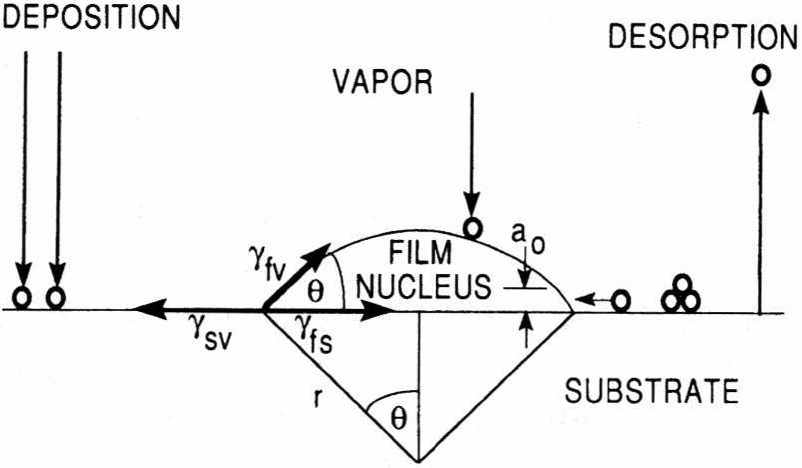
\includegraphics[width=0.7\textwidth]{back_rates}
    \caption{\label{fig:back_epi_rates}Processes with kinetic rates during epitaxy}
\end{figure}

The most common experimentally controlled rates in an epitaxial growth are the rate of addition of atoms to the growth interface, and the rate the temperature is increased or decreased during a growth. The rate of atom addition, or the growth rate is a key parameter and in homoepitaxial growth, can reveal the role kinetics plays in growth. If the rate at which atoms are added to an epitaxial interface is extremely high, the atoms will have no time to move towards their thermodynamically preferred location. The resulting material that grows will consist of the layers of atoms stacked randomly where they first hit the substrate and were immediately covered by more atoms. Such a configuration is clearly not an epitaxial growth, rather the film is likely to be amorphous, yet there are no material limitations per-se that causing the poor growth, it is purely kinetic. As the growth rate is lowered adatoms are allowed more time to move via diffusion, they may register in some regions, but not in others, resulting in a partially crystalline growth. As the deposition rate is further reduced, depending upon the material, the film may grow in a fully crystalline nature, but be twinned or contain stacking faults. The bonding along \{111\} directions in a crystal susceptible to faults due to their relative rotational symmetry, the exact susceptibility is known by the Stacking Fault Energy (SFE)\cite{stacking-fault-energy}. This energy is a measure of the cost of making such a defect in a crystal, so crystals with low SFE are very susceptible to twinning during growth. As the growth rate is still lowered, the adatoms have time to find their low energy states with respect to twins, finally arriving at a single crystal.
\begin{equation}
A = A_0 \exp^{-\frac{E_0}{kT}} \label{eqn:arrhenius}
\end{equation}
While the directly controlled deposition rate seems to be severely limited by defect formation and stacking of adatoms, there are large number of kinetic processes during growth that can be indirectly influenced by an experimenter through the control of temperature. Fundamentally, the other kinetic processes fundamental to growth are all of the Arhennius type, as shown in\cref{eqn:arrhenius}. As such, these processes have an exponential dependence on the temperature at which growth occurs. Among the other kinetic processes involved in growth, the most important are surface diffusion, bulk diffusion, desorption and nucleation/denucleation. Through the increase in temperature the rates of all of these (except nucleation) processes increases. This has a strong impact on the epitaxial process. 

The key kinetic factor to the improvement of epitaxial growth is the increase in the surface diffusion rate. Surface diffusion of adatoms during growth is the process by which an newly adsorbed atom from the impinging atoms finds its lowest energy position on the epitaxial surface. Increases in temperature increase the rate at which these adatoms move, increasing the probability that they will find their lowest energy position before they are encapsulated by additional atoms. While increases in temperature will improve the mobility of adatoms, increases in temperature also increase other processes. Bulk diffusion is the process by which adatoms at the epitaxial interface diffuse into the bulk through exchange with other atoms or travel interstitially. In homoepitaxy this process is mostly irrelevent, but in any chemically dissimilar growth such a process distorts the interface, which is generally not preferred. Similarly, as temperature increases, the adatoms begin to desorb, leaving the epitaxial interface, slowing growth and under extreme circumstances, the substrate itself can also begin to breakdown. Finally, at very high surface diffusion rates, adatoms may not ever attach to others, nucleating new layers of crystal.

The kinetics of growth are thus balanced between the intended growth rate, determined by the delivery of atoms to the epitaxial interface, and a temperature that is high enough to ensure single crystal growth, but not too high as to cause breakdown of the epitaxial process itself.

\todo{Reference some work on Silicon-Silcon homoeptiaxy which demonstrates these facts}


\subsection{Heteroepitaxy}
Heteroepitaxy covers a wide range of A on B epitaxy systems, as such, the following treatment will start from the basics established in homoepitaxy and gradually add the levels of complexity found in real-world systems and consider how they add to the model.

\subsubsection{Strained Heteroepitaxy}
The first step in the complication from homoepitaxy to heteroepitaxy is to introduce a difference in the lattice constants between the substrate and the growing epitaxial crystal, while maintaining the crystal structures and chemical composition. Nature has provided an ideal model system which perfectly fits these requirements, the Si$_{1-x}$Ge$_x$ system grown on silicon. In Si$_{1-x}$Ge$_x$, germanium substitutes into the silicon lattice randomly, maintaining the same valence and diamond structure. The lattice constant varies nearly linearly between silicon and germanium as in \cref{eqn:sige}.
\begin{equation}
a_{Si_{1-x}Ge_x} = 0.5431 + 0.01992x + 0.0002733x^2 \label{eqn:sige}
\end{equation}

The difference between lattice constants is expressed as the lattice mismatch as in \cref{eqn:mismatch}. Negative values indicate that the growing layer is in tension by bonding to the substrate, while positive values indicate that growing layer is in tension by bonding to the substrate. The fundamental physical parameter describing such mismatched system is strain, this is, the distortion of atoms from the thermodynamic equilibrium positions, due to bonding to a mismatched substrate. Strain can be conceptualized as energy stored within the stretched bonds of the epitaxial layer, increasing the internal energy within the epitaxial crystal.
\begin{figure}
    \centering
    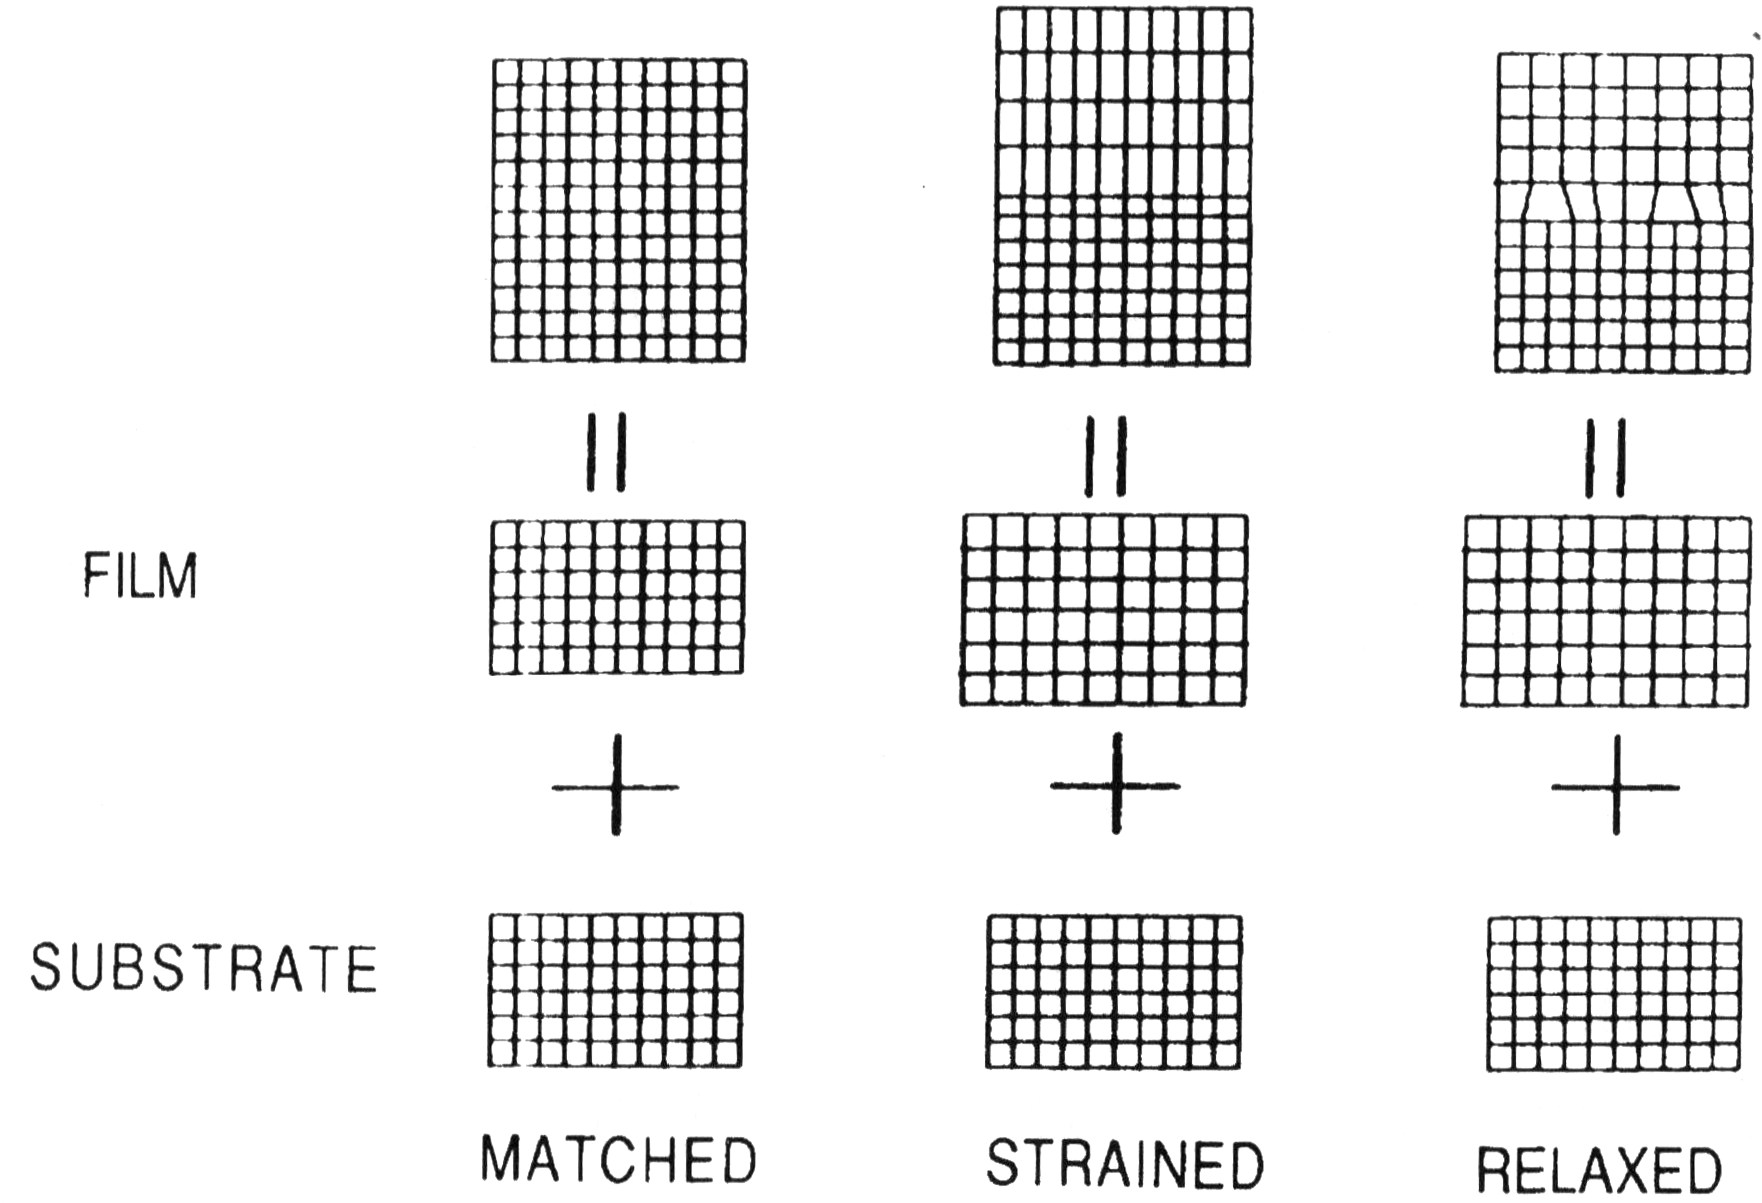
\includegraphics[width=0.8\textwidth]{back_strain}
    \caption{\label{fig:back_strain}Unit cell models of matched, strained and relaxed films from \cite{ohring2001materials}}
\end{figure}

Through the examination of the Si$_{1-x}$Ge$_x$ system grown on silicon, the effect of pure compressive strain on an epitaxial process has been examined. As an epitaxial crystal of Si$_{1-x}$Ge$_x$ is grown on a silicon substrate, the strain energy in the crystal increases with thickness. The growing epitaxial crystal maintains the lateral lattice constant of the substrate, and conserves it's volume by changing it's vertical lattice constant, this is known as pseudomorphic growth. Beyond a certain point, the energy required to add another layer of strained crystal is too much, and the strain is relieved through the introduction of a defects in the form of dislocations. In a dislocation, the bonding between the epitaxial crystal and the substrate is broken to allow the crystal to expand, leaving a dangling bond at the substrate. Such a process is random so defects are located randomly at the interface. The exact thickness where a pseudomorphic growth will introduce defects in order to accommodate strain is known as the critical thickness and is dependent upon a number of factors including the strength of the bonds across the epitaxial interface, the bond strength within the epitaxial layer, and the energetic cost of forming a dislocation in terms of atomic movement and dangling bonds. The experimental curve for the model system Si$_{1-x}$Ge$_x$  is shown in \cref{fig:back_strain_regions}. The critical thickness model is qualitatively similar for other systems that have similar growth properties.
\begin{equation}
f = \frac{a_f - a_s}{a_s} \label{eqn:mismatch}
\end{equation}
\begin{figure}
    \centering
    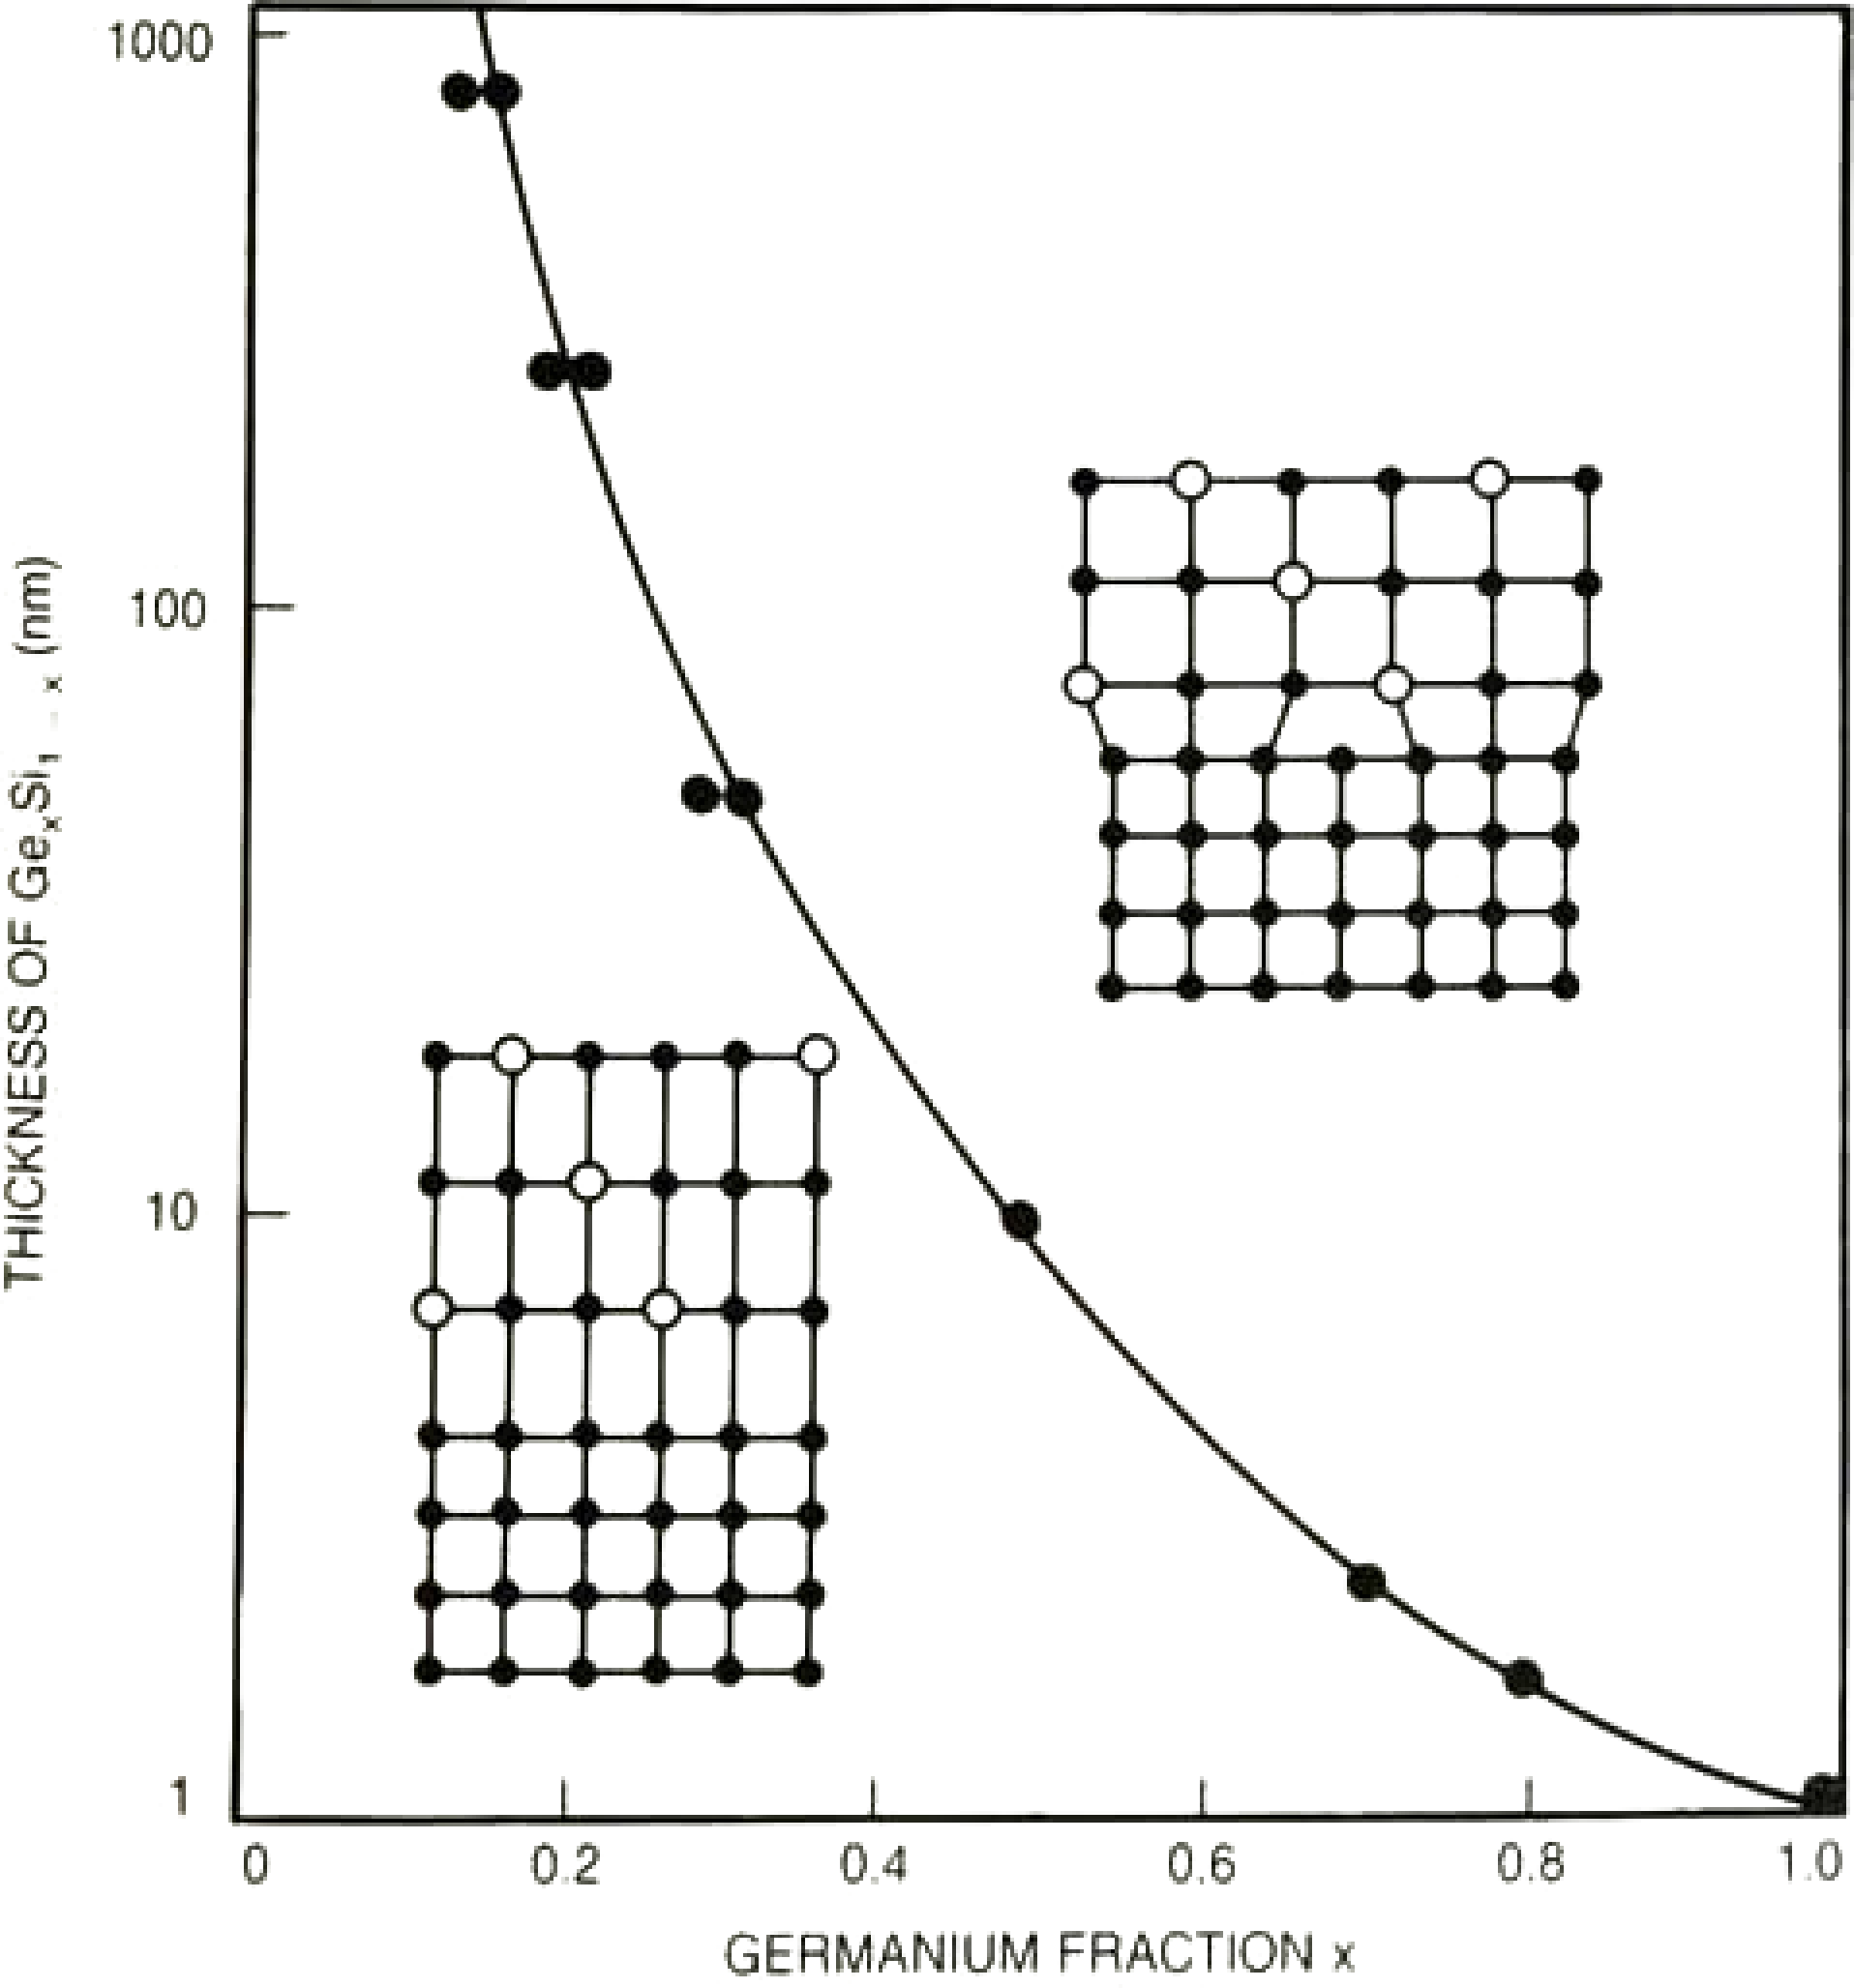
\includegraphics[width=0.6\textwidth]{back_strain_regions}
    \caption{\label{fig:back_strain_regions}Regions of pseudomorphic and relaxed growth versus lattice mismatch\cite{Bean1986}}
\end{figure}
\subsubsection{Chemically Dissimilar Heteroepitaxy}
On the other side of the heteroepitaxy spectrum are those epitaxial growths that have identical crystal structures but differ in their chemical compositions. There few material systems which provide an ideal model for a lattice matched (zero strain), but chemically dissimilar epitaxial growth. The most well characterized model system available is a lattice matched III-V semiconductor on germanium, specifically GaAs, which has an extremely small ($<$0.1\%) lattice mismatch. GaAs is a binary semiconductor with a the zinc blende structure, which is a cubic crystal identical to silicon and germanium's diamond structure, but with a two-atom basis (Ga, As). The crystal is covalently bonded as with Si, but has a $\sim$30\% ionic character due to differences in electronegativity\cite{Christensen1987}.

The zinc blende crystal structure is due to the presence of two atoms of different valence (group III-group V), which forms a polar crystal structure, with the group-III atom supplying three electrons and the group-V atom supplying five electrons to the bonding structure. The two-atom basis of zinc blende breaks the diamond crystal structure such that the structure is no longer centrosymmetric, meaning that opposite directions in the crystal are no longer symmetrically equivalent. This breaking of symmetry in the crystal means that the ordering of the group-III and group-V atoms at the epitaxial interface matters for crystal growth. This problem is known as ``polar-on-nonpolar'' epitaxy\cite{Biegelsen1992,Kroemer1987}.
\begin{figure}
    \centering
    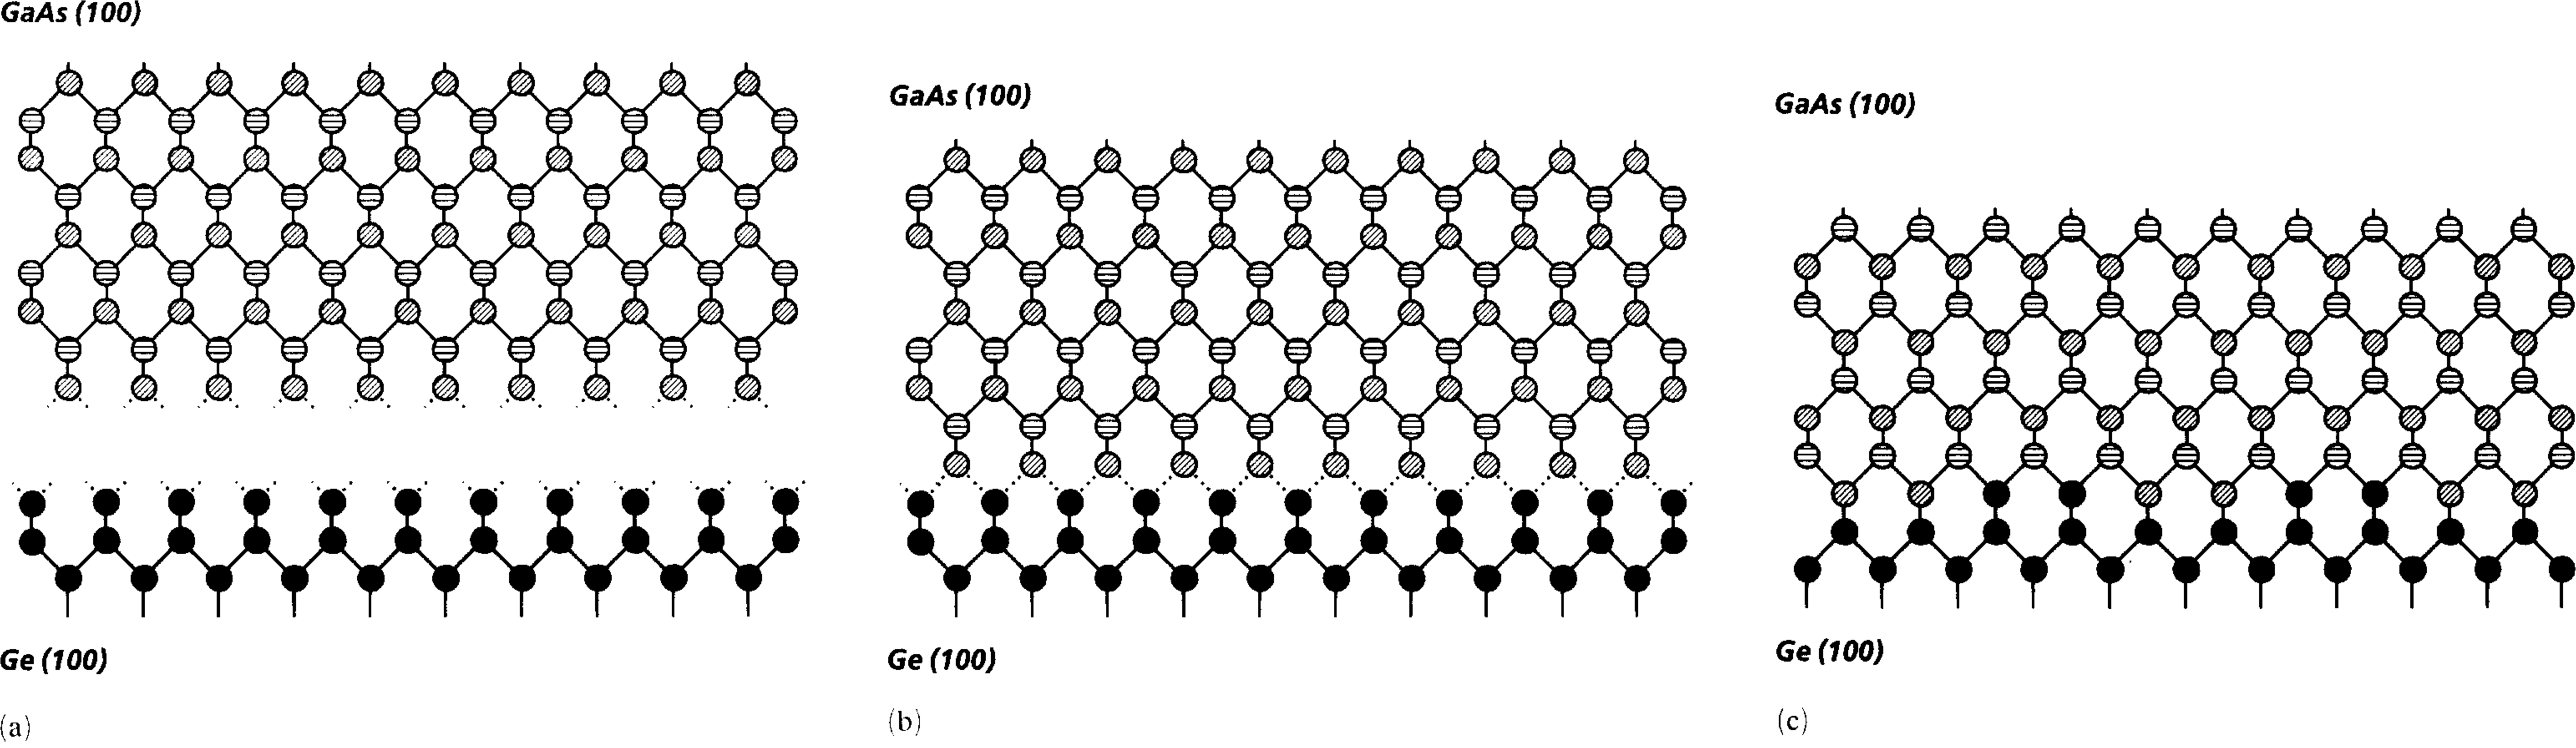
\includegraphics[width=\textwidth]{back_polar_model}
    \caption{\label{fig:back_polar_model}Ideal polar on non-polar after \cite{Biegelsen1992}}
\end{figure}

If the truncated crystal surface of such a polar semiconductor is brought towards the truncated surface of a silicon crystal as in \cref{fig:back_polar_model}, the interface that results, while all bonds will be satisfied with no strain, will not be satisfied electronically. There will be an excess or deficit of electrons participating in bonding at the interface, leaving a layer of excess charge. Such excess charge would be massive as it forms across the entire interface. During growth of a crystal, rather than the thought experiment just discussed, we could expect that the surface charge would be a driving force for an atomic rearrangement at the interface. Experimental results have shown that a number of rearrangements are possible. The interface region can become three dimensional with the substrate and epitaxial layer atoms swapping in order to balance the number of excess and deficient bonds, resulting in an overall neutral charge. Various defects can also form, resulting in dangling bonds which can compensate charge. Some orientations of the crystal substrate, such as (211) offer unique lattice sites such that the charge neutrality is maintained automatically, which has motivated some of the work presented in \cref{sec:211}.

In addition to issues of charge neutrality at chemically dissimilar ideal epitaxial interfaces, there are is a second common issue that arises. This issue only arises in practical growth situations, due to the fact that real substrates are never perfectly aligned with their intended crystal orientation. These substrates, when offcut even the smallest amount, will reconstruct into terraces of the primary crystal orientation separated by atomic height steps, the details of this process will be covered in \cref{sec:reconstruction}. When those steps are single steps, that is, a/2 in height, adjacent terraces expose different sublattices of the diamond structure and these two sublattices have their exposed bonds rotated relative to each other. When a crystal is grown atop such a substrate, the growth on adjacent crystals will also be offset by a/2. While such an offset is not detrimental to the substrate itself, the zinc blende crystal structure with two different atoms, when offset by the same amount, will result in a misalignment of the growing crystal at the step edges. The step edge will contain III-III or V-V bonds, a section known as an anti-phase boundary, a defect that causes significant electrical defects and unintentional doping due to uncompensated bonds. Sufficient care must be taken when preparing substrates (as noted later in \cref{sec:reconstruction}) in order to avoid these highly detrimental anti-phase boundaries.

\todo{Find calculation/figure of step formation versus offcut angle}
\subsection{Clusters and Nucleation}
As will arise again and again throughout this document, the key factor in the growth of epitaxial crystals is the properties of the epitaxial interface. The two generalized properties that impact this interface are the energy and symmetry at the interface. The initial stages of the epitaxial growth process is a key step which reveals the complex interplay of strain, energy and symmetry, through the form of the nucleation of the epitaxial crystal.

A key qualitative measure of the affinity of a given crystal to grow on another crystal is what is termed the nucleation mode of the epitaxial crystal. Qualitatively, the nucleation mode of a given epitaxial crystal \textbf{A} on a substrate \textbf{B}, describes the affinity for the atoms in \textbf{A} to wet (spread out and contact) the substrate versus sticking to each other. The wetting and dewetting of a given system is described by Young's equation, as in \cref{eqn:youngs}. Young's equation describes the balance of three energies, the film-substrate energy, the substrate-vapour energy and the film-vapour energy, through a parameter denoted the contact angle. The contact angle is the key parameter which determines wetting characteristics of a system.
\begin{equation}
\gamma_{FS} + \gamma_{FV} \cos{\theta_c} = \gamma_{SV} \label{eqn:youngs}
\end{equation}
Young's equation can be visualized as a droplet of the epitaxial crystal material sitting atop a substrate, making some contact angle with the substrate, as in \cref{fig:back_epi_young}. Contact angles of less than 90\degree{} are denoted as wetting a surface, while angles greater than 90\degree{} are denoted as dewetting a surface. During epitaxial nucleation, incoming atomic material grows as one of three modes, named island nucleation, layer-by-layer nucleation, and stranski-krastanov or mixed-mode nucleation, as in \cref{fig:back_growth_mode}. 
\begin{figure}
    \centering
    \missingfigure{Young's equation visiulaization}
    \caption{\label{fig:back_epi_young}Young's equation visualized as a droplet sitting atop a substrate}
\end{figure}

The energies in Young's equation are intrinsic to the crystal and chemical relationship between the epitaxial crystal and the substrate, as well as possibly the overlying gas. Strain and chemical bonding are the two primary factors which influence the energy parameters which participate in the nucleation process. The regions of have been mapped experimentally for several model systems, both chemically similar and strained, and the chemically dissimilar but unstrained, as shown in \cref{fig:back_nucleation_regions}. Layer-by-layer nucleation and growth is most readily achieved when the epitaxial crystal and substrate are chemically compatible and have minimal strain. For chemically incompatible systems nucleation is always island nucleation, as the epitaxial crystal would rather bond to itself than the substrate. With increasing strain nucleation can begin as layer by layer, but transition to island after several layers.

 In general, there are other factors not considered as part of this simple model. The model does not directly consider the crystalline nature of the growing layer, such as its preference for the island facet into low energy surfaces. These nucleation modes also do not consider the kinetics of the growth process, if atoms are delivered too quickly nucleation can form islands regardless of the predictions of Young's equation.
\begin{figure}
    \centering
    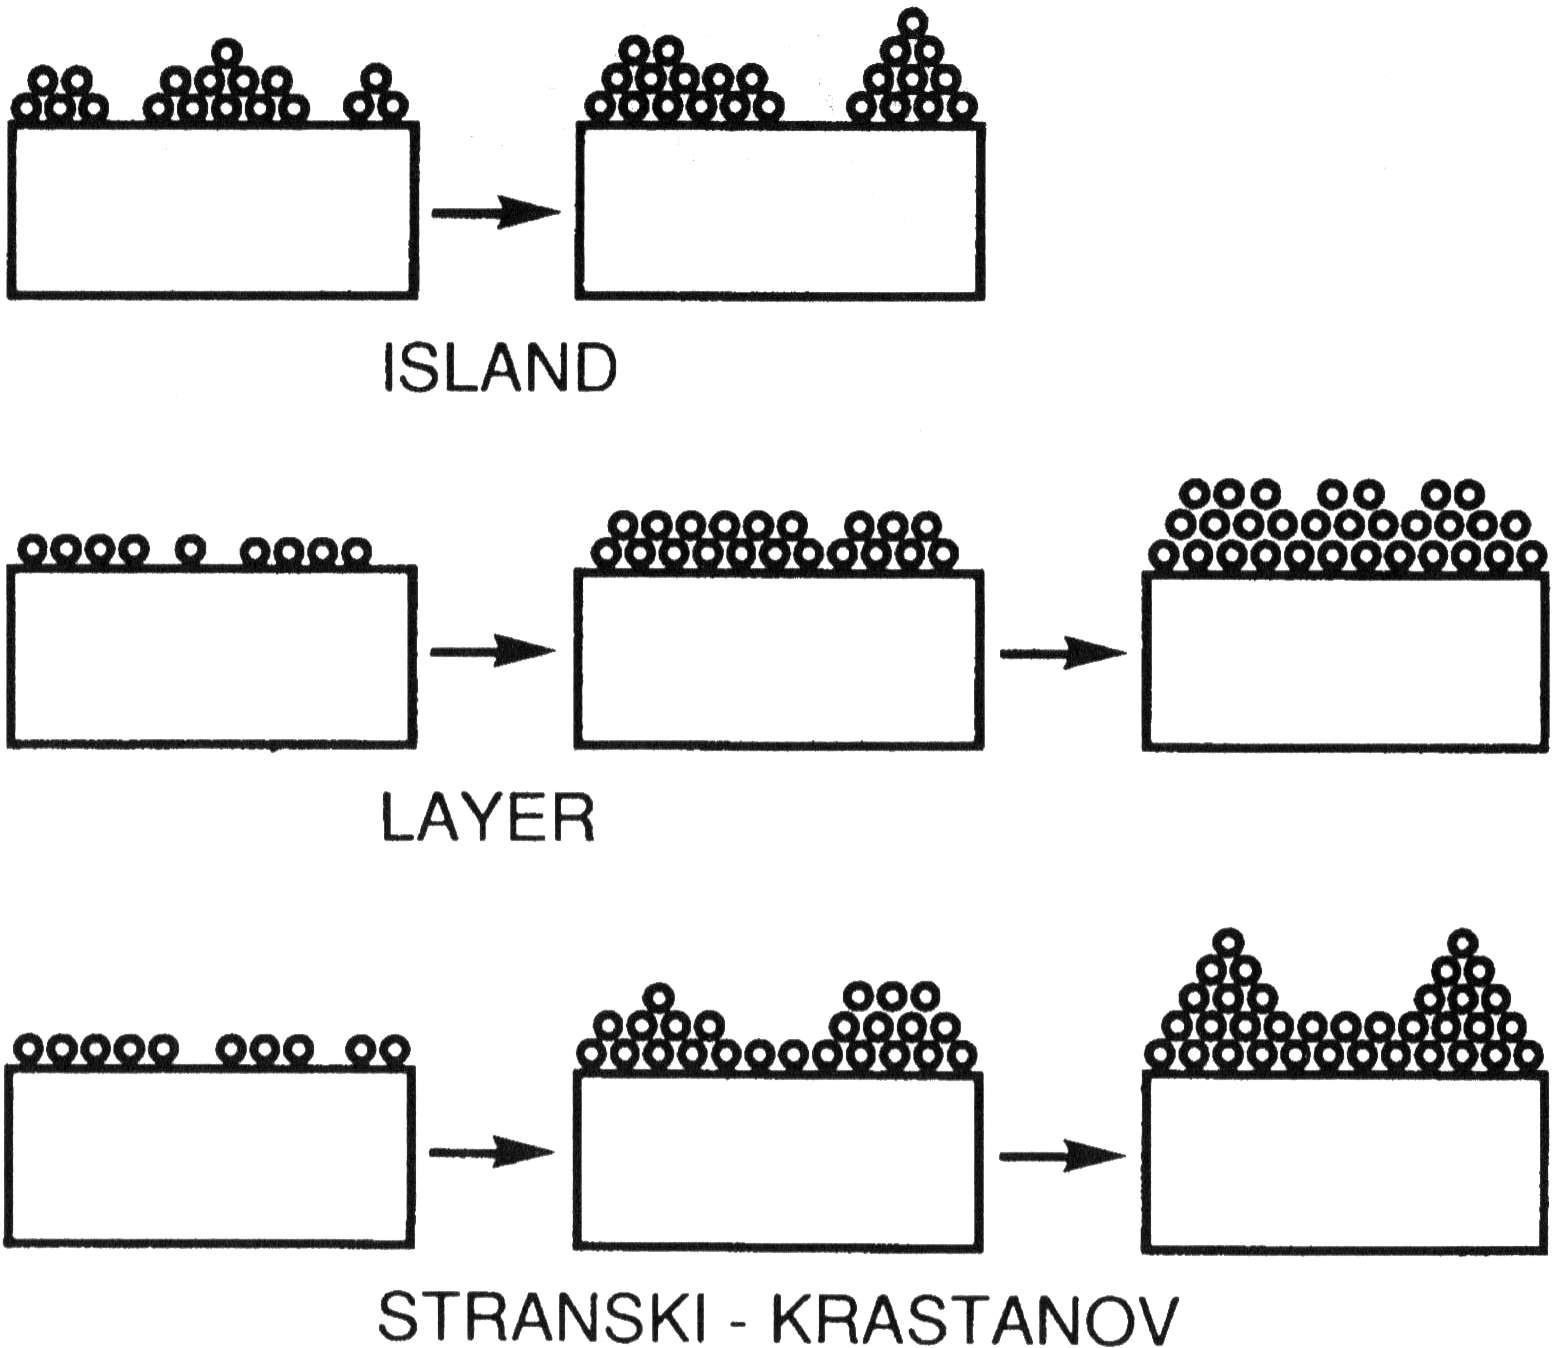
\includegraphics[width=0.6\textwidth]{back_growth_mode}
    \caption{\label{fig:back_growth_mode}SK, layer-by-layer and frank van der mere growth modes\cite{ohring2001materials}}
\end{figure}

\begin{figure}
    \centering
    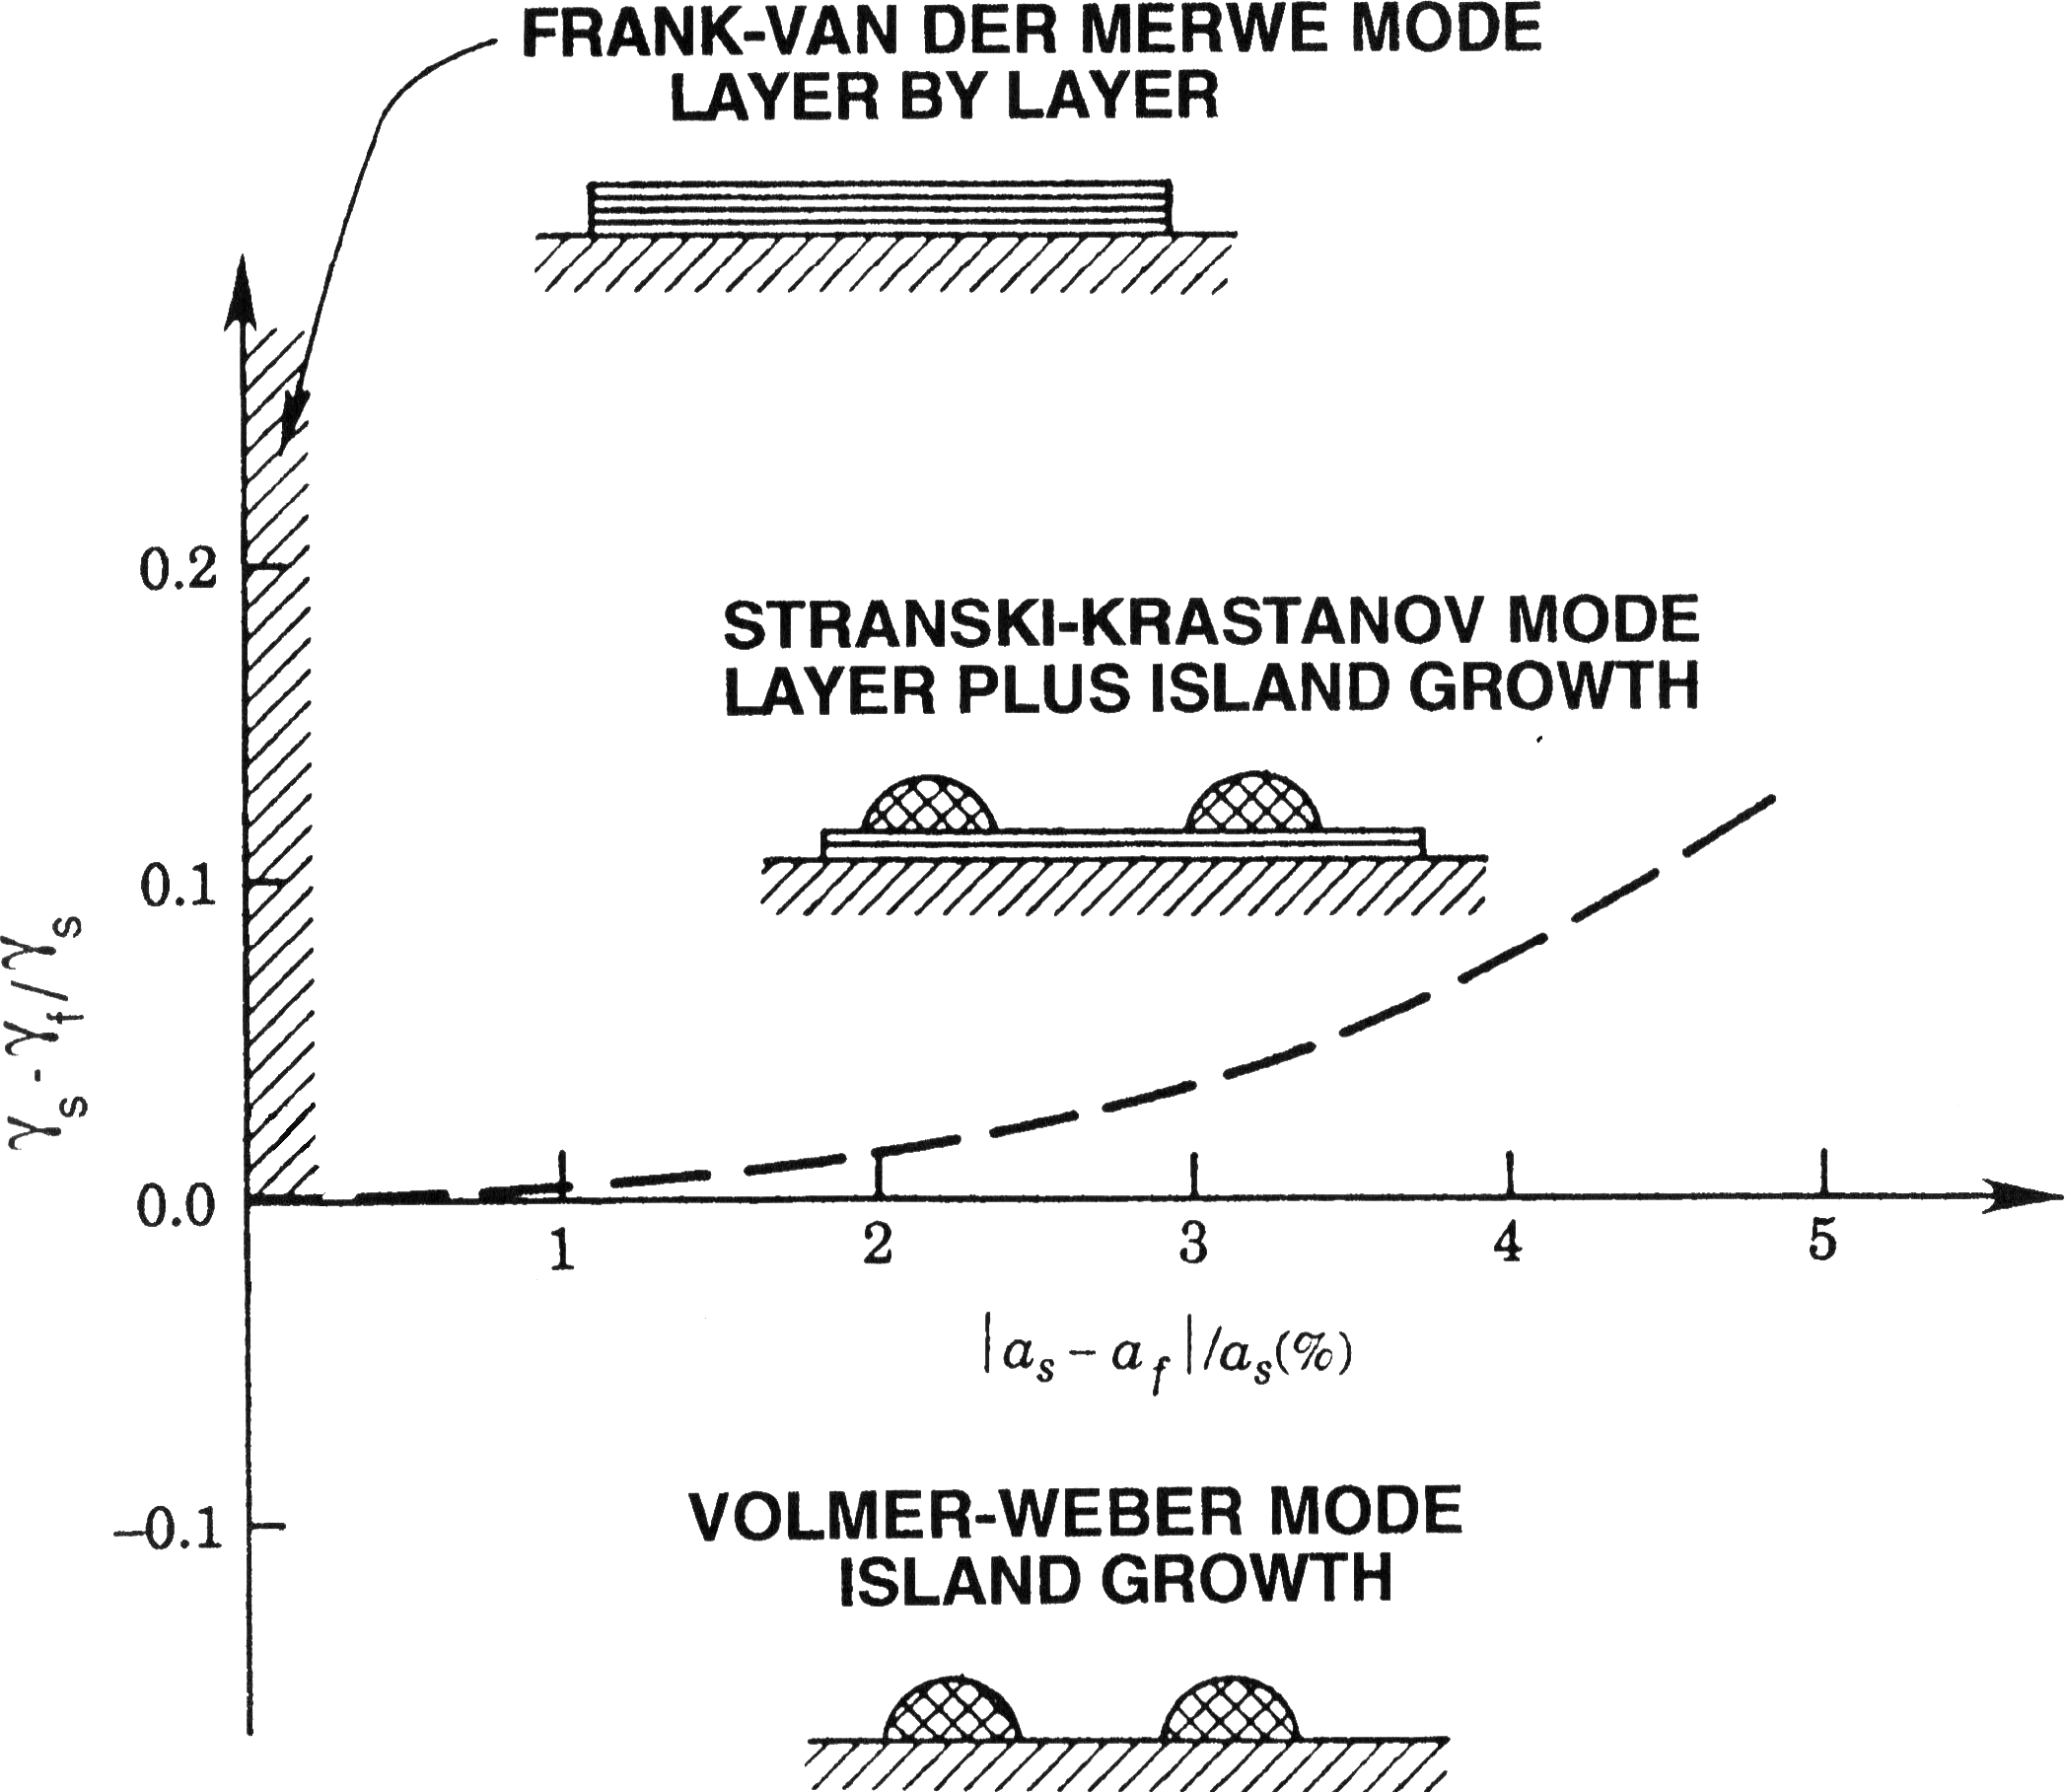
\includegraphics[width=0.7\textwidth]{back_nucleation_regions}
    \caption{\label{fig:back_nucleation_regions}Regions of different nucleation/growth modes as a function of lattice mismatch and surface energies\cite{ohring2001materials}}
\end{figure}

\section{Surface Reconstructions}\label{sec:reconstruction}
If one were to consider a crystal of infinite size, and subsequently cut it along any direction, the resulting surface would be a very high energy surface. Bonds will be completely unsatisfied (truncated electron clouds), there is likely to be an unbalanced charge, and the surrounding environment for each surface atom will be significantly different than they were in the bulk. This high energy condition is clearly not the equilibrium state and must be resolved. The resolution of this high energy state that results when surfaces of a single crystal are exposed is called the surface reconstruction. While the name surface reconstruction implies changes to just the surface atoms, the surface reconstruction can extend a number of layers into crystal. Thus, the changes that occur at the surface of a crystal can result in a very different interface than the bulk crystal for the purposes of epitaxy.

The atoms on the surface of a newly cleaved crystal have a number of options for resolving their high energy configuration. The simplest of options for atoms in those high energy states to reduce their energy is to move, that is, to change it's position relative to other atoms. These movements happen both the in-plane and out-of-plane directions. Both atomic translations can cause additional shifts in the atomic layers below the surface.  Both in-plane and out-of-plane atomic movement breaks the bulk symmetry of the original crystal, resulting in a surface with lower symmetry. In extreme cases, atoms can migrate and form islands or otherwise cause faceting on the surface in order to minimize energy. A schematic example of the atom movement for surface reconstruction is shown in \cref{fig:back_recon_move}.
\begin{figure}
    \centering
    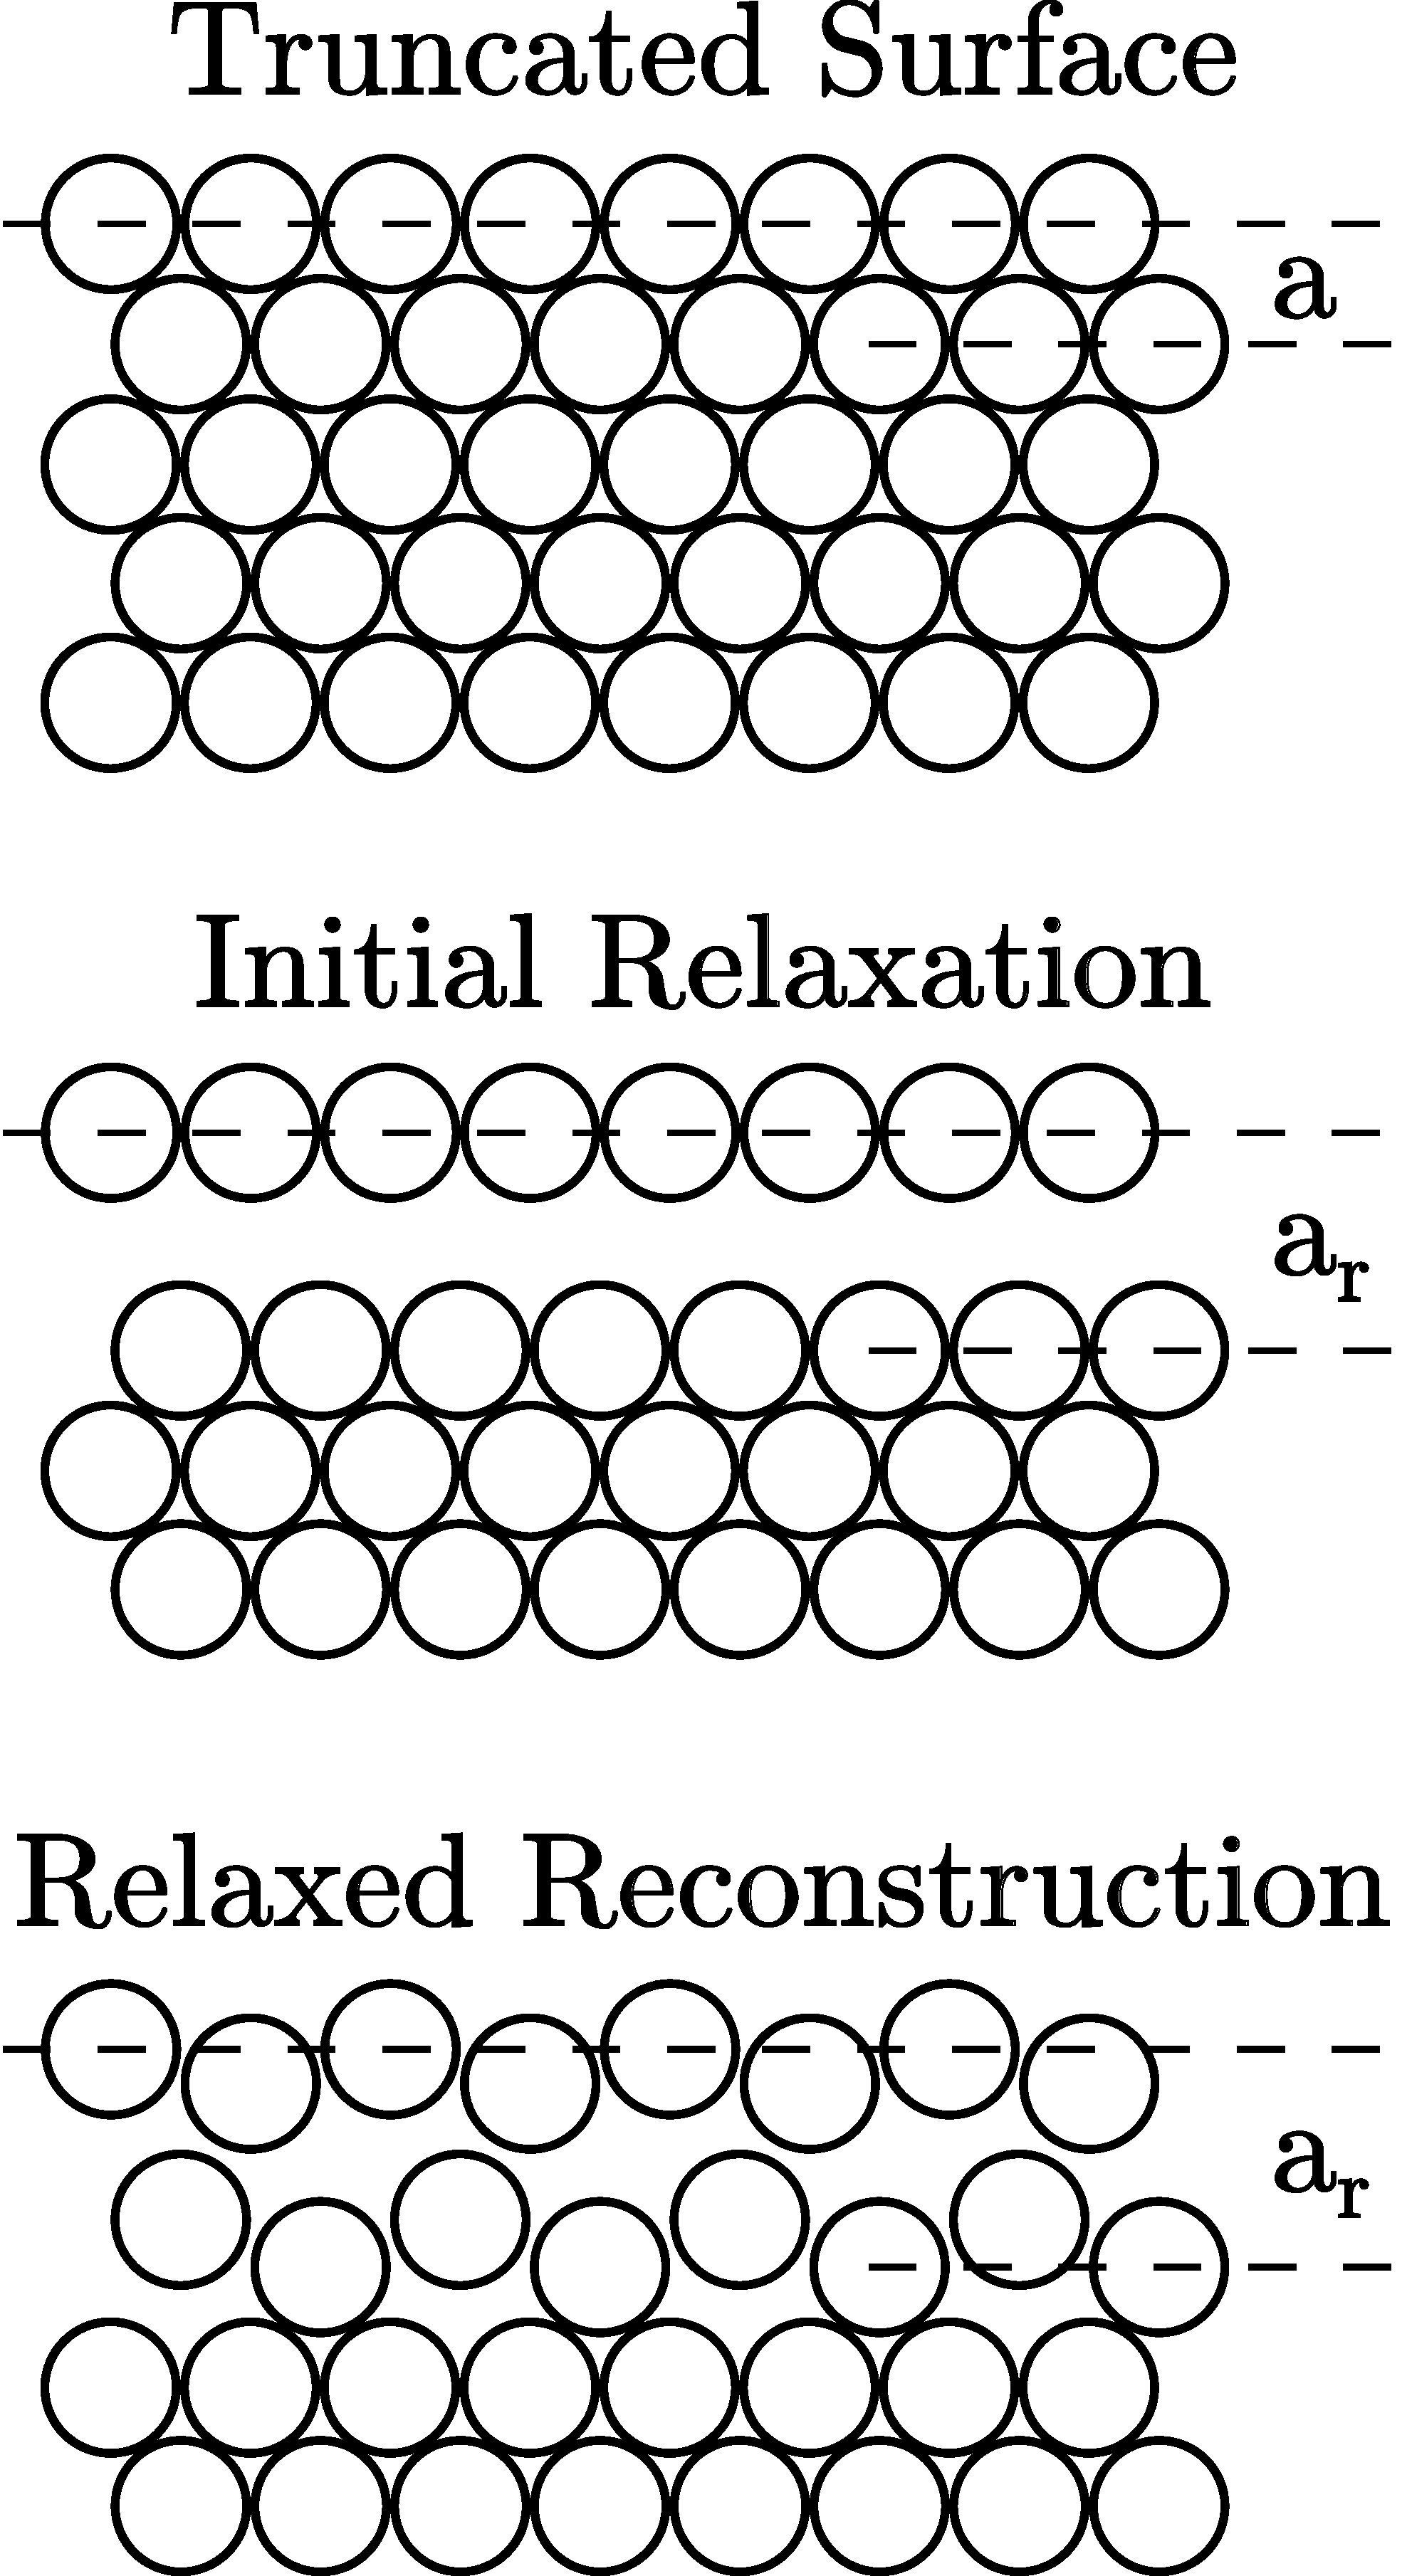
\includegraphics[width=0.5\textwidth]{back_recon_move}
    \caption{\label{fig:back_recon_move}Example of surface reconstruction with atomic movement\cite{ohring2001materials}}
\end{figure}

A more complex response resulting in a surface reconstruction that can arise is a change in the actual bonding in the upper layers of the crystal. Dimers and higher order bonding can form at the surface of the crystal, partially resolving the dangling bonds present on the surface. This dimerization of the surface can significantly reduce the chemical activity of the surface since the electronic structure has been satisfied internally to the crystal. An example of such dimerization is shown in \cref{fig:back_recon_dimer}
\begin{figure}
    \centering
    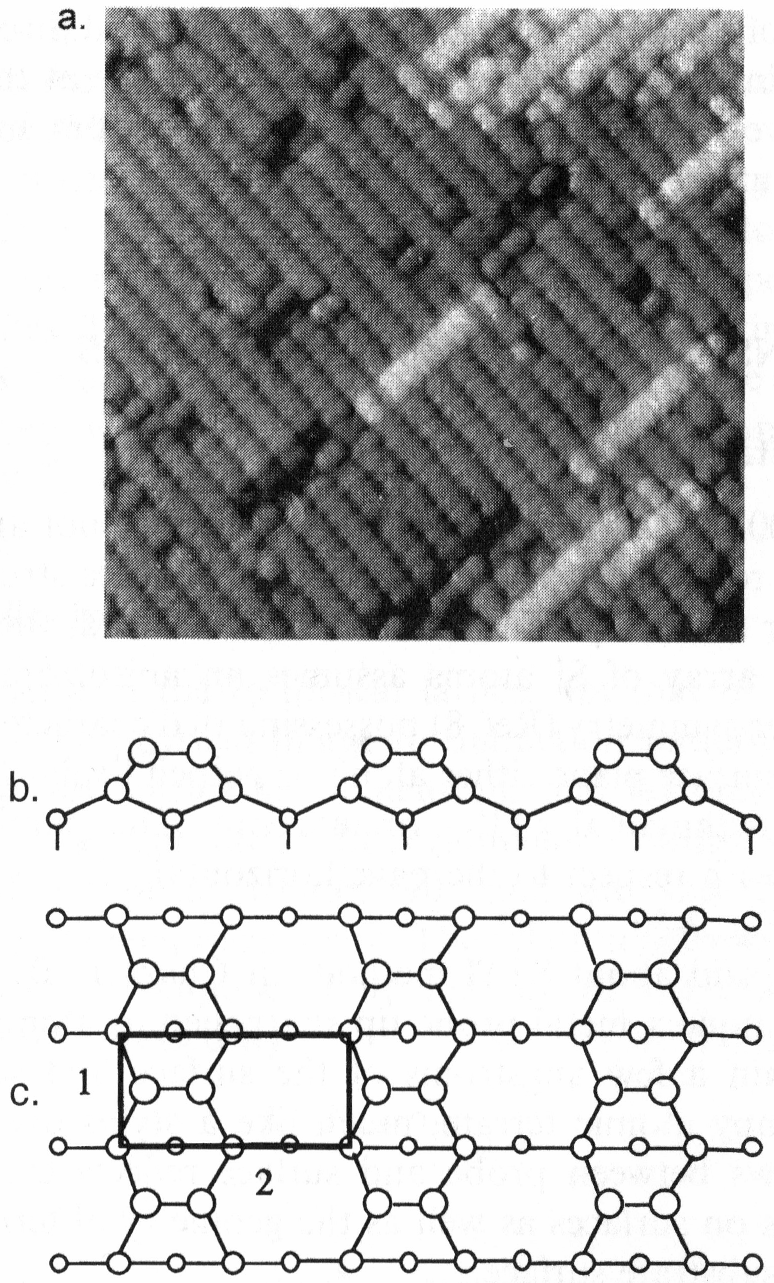
\includegraphics[width=0.7\textwidth]{back_recon_dimer}
    \caption{\label{fig:back_recon_dimer}a) STM of silicon surface reconstruction showing dimers b) cross sectional view of model ($2 \times 1$) surface reconstruction c) top view showing reconstructed surface unit cell \cite{ohring35}} 
\end{figure}

Finally, a surface can reconstruct by losing some of the atoms which originally formed the surface. The removal of such atoms can allow which was once a close-packed surface to have significantly less density than the parent crystal lattice.

\subsection{Cuts along high-index planes}
When crystals are cut along low index planes (100,111,110), surface reconstructions happen directly on these surfaces. When crystals are cut along high index planes, there is additional energy associated with exposing non-close-packed planes. These high index planes are highly unfavourable and do not have stable reconstructions. The high index surface instead undergoes a breakup into sections of low index planes, separated by steps of fractional or multiples of the unit cell, as shown in \cref{fig:back_recon_vicinal}. These low index planes can then further reconstruct as previously discussed.
\begin{figure}
    \centering
    \missingfigure{Vicinal surface showing reconstruction}
    \caption{\label{fig:back_recon_vicinal}Vicinal surface showing reconstruction}
\end{figure}

The most common case of high index planes exposed for surface reconstruction is offcut or vicinal surfaces. The surfaces of single crystal wafers, when cut from a boule have a misalignment from the intended low-index plane due to processing error. These wafers, when reconstructed form terraces of the low index plane, separated by fractional unit cell steps.

\subsection{Thermodynamics, Kinetics and Stability of Surface Reconstructions}
While a unreconstructed crystal surface is in a high energy state, all the routes to lower energy states require an input of energy. Thus, while a crystal surface may be in a relatively high energy state after cutting, cleaving, polishing or other processing which exposes that surface, it can do very little to resolve its situation without help. Energy must be inputted into the system in order to allow the atoms to move, bond or leave the surface. The energy landscape of surface reconstructions has many local minima, so there are many possible surface reconstructions for a given surface, depending upon how much activation energy is provided to the system. Beyond how much energy is delivered to the crystal, it takes time for the atoms to reach a one of local minima for the surface. Some surface reconstructions can take a significant time to achieve, adding more energy would result in transitions into another reconstruction so the only route is time.

Thus far, energy and time have only been discussed in general terms. The most successful and commonly used method of actually delivering energy and eliciting a reconstruction is to increase the temperature of the crystal. Annealing crystals can be done at a carefully controlled temperature for any desired amount of time. Careful experimentation with various crystals has resulted in ``phase diagrams'' of surface reconstructions given a surface and temperature combination, as seen in \cref{fig:back_recon_phase}.
\begin{figure}
    \centering
    \missingfigure{Phase diagram of surface reconstruction}
    \caption{\label{fig:back_recon_phase}Phase diagram of surface reconstruction}
\end{figure}

The formation and stability of a given surface reconstruction also depends upon the environment surrounding the crystal. Assuming the surrounding environment does not chemically react with a given crystal, the presence of absence (vacuum) of an inert gas will affect the activation energies for the surface atom processes. A vacuum above a crystal when annealing promotes the exit of atoms from the surface as there is force resisting the atoms, or back scattering them towards the surface. For complex crystals which incorporate elemental gasses into their lattice, different surface reconstructions are achievable if an overpressure of those gasses are present, rather than a vacuum. These surface reconstructions are commonly seen in the complex oxides, where oxygen is a primary constituent of the crystal and will be lost from the surface during annealing if an overpressure is not provided.

Stability of surface reconstructions to subsequent interactions with atoms added to the surface varies widely depending upon the properties of the crystal. Semiconductor crystals have less stable surface reconstructions, interactions with additional atoms easily destroy an established reconstruction. Refractory crystals such as complex oxides are considerably more stable once reconstructed, a point which has been taken advantage of in this work.

\subsection{Nomenclature for Surface Reconstructions}
Since surface reconstructions are pseudo-2D constructs, the allowed symmetries of a surface reconstruction are a subset of those of the allowable 3D lattices. There are five unique 2D surface nets that can be used to describe the symmetry of a surface reconstruction as shown in \cref{fig:back_recon_lattices}
\begin{figure}
    \centering
    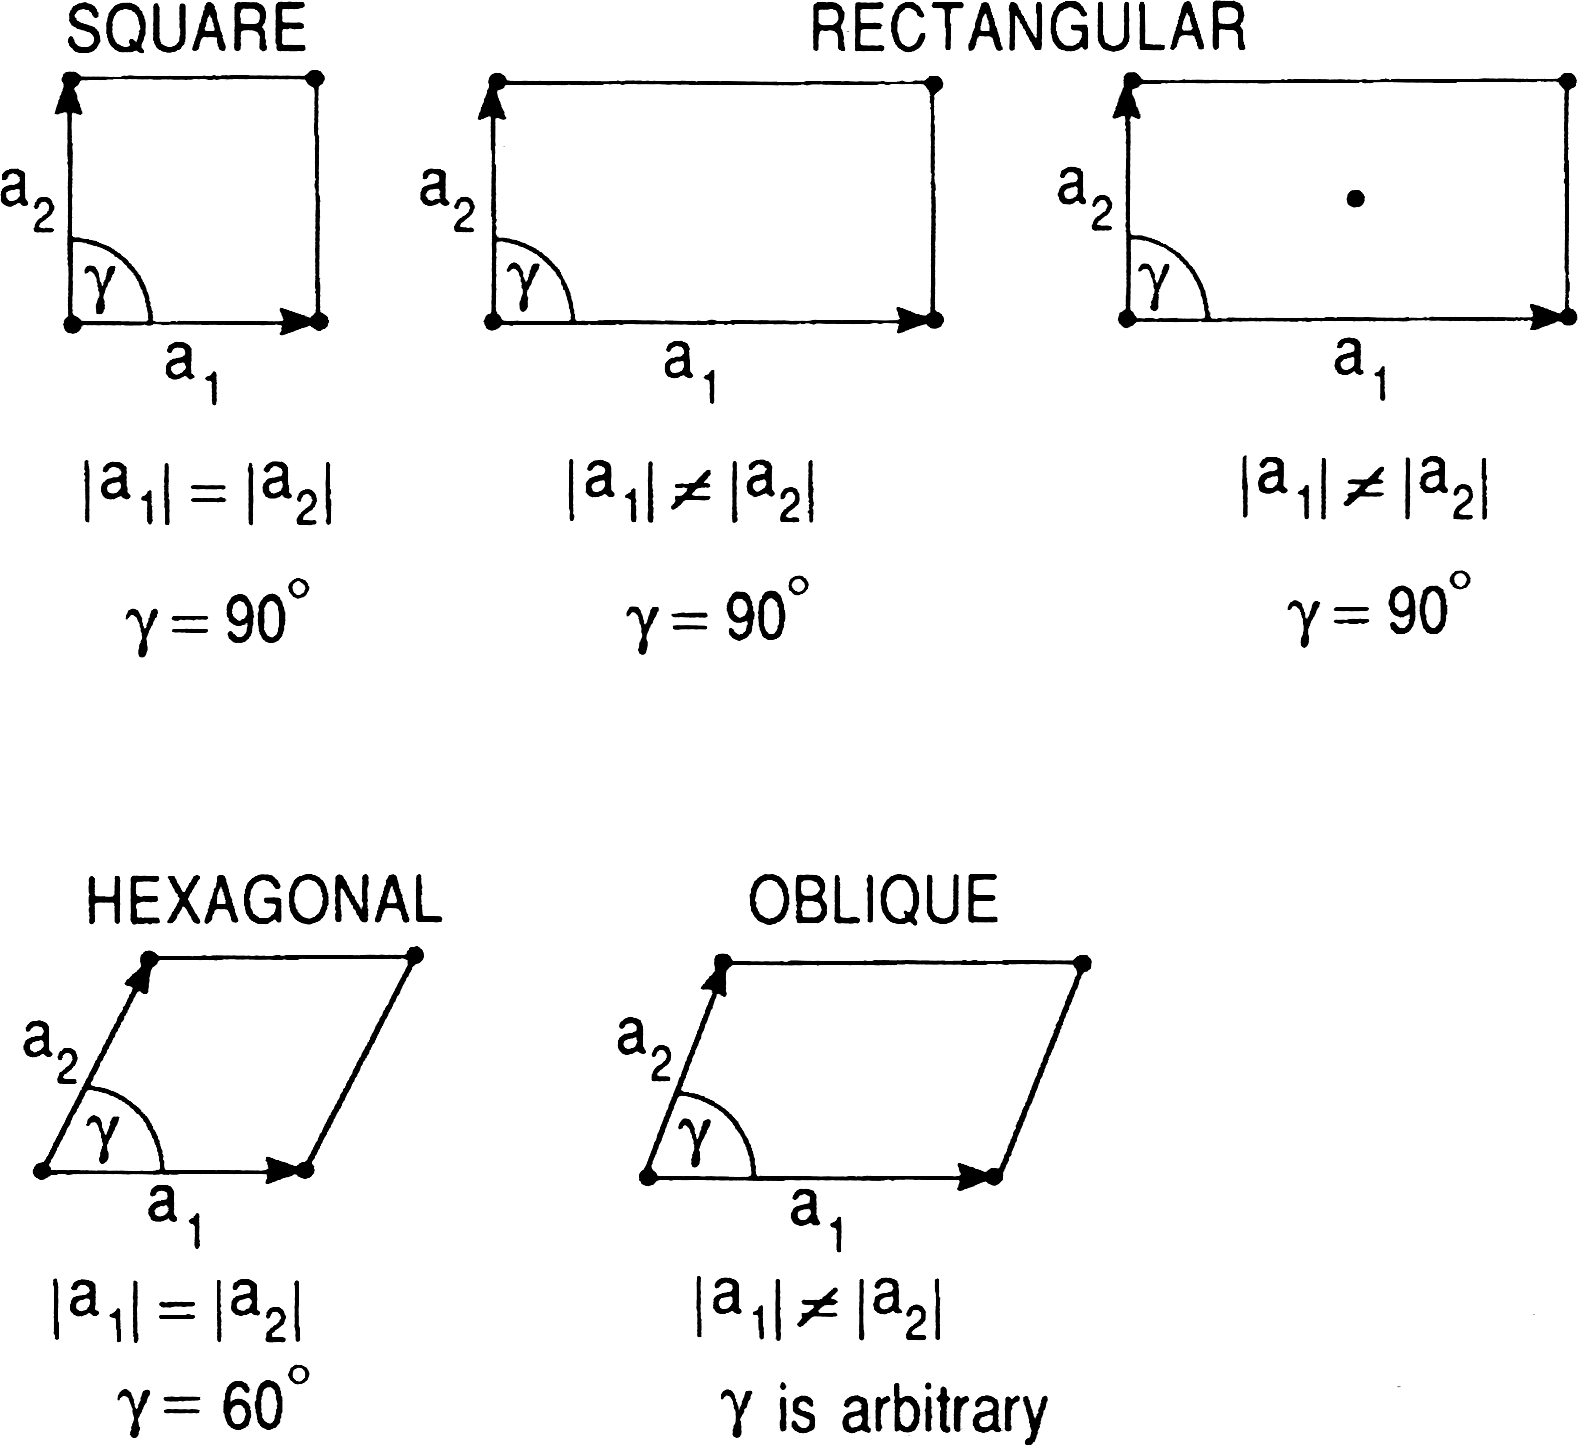
\includegraphics[width=0.8\textwidth]{back_recon_lattices}
    \caption{\label{fig:back_recon_lattices}The five unique 2D surface nets\cite{ohring2001materials}}
\end{figure}

The nomenclature of naming surface reconstructions is determined by the relationship of the 2D surface lattice to the underlying unit cell. The smallest repeating surface cell is determined and denoted by whether it is primitive (P), having only one atom per surface cell, or centred (C). The surface cell's repeat unit is then related to underlying unit cell by the ratio of the surface cell lattice constant to the unit cell lattice constant. Thus, the simplest surface reconstruction for a crystal would be the P($1 \times 1$) reconstruction, containing one atom, and having the same spacing as then underlying crystal. These nomenclatures do not include details such as the type, number or configuration of atoms which make up the reconstruction. These reconstructions can also be rotated relative to the underlying unit cell being denoted by R. A number of example surface reconstructions namings are shown in \cref{fig:back_recon_name_examples}. The nomenclature for surface reconstructions is not unique, as a reconstruction such as C($2\times2$) is equivalent to ($\sqrt{2}\times\sqrt{2}$)R45\degree~reconstruction.
\begin{figure}
    \centering\
    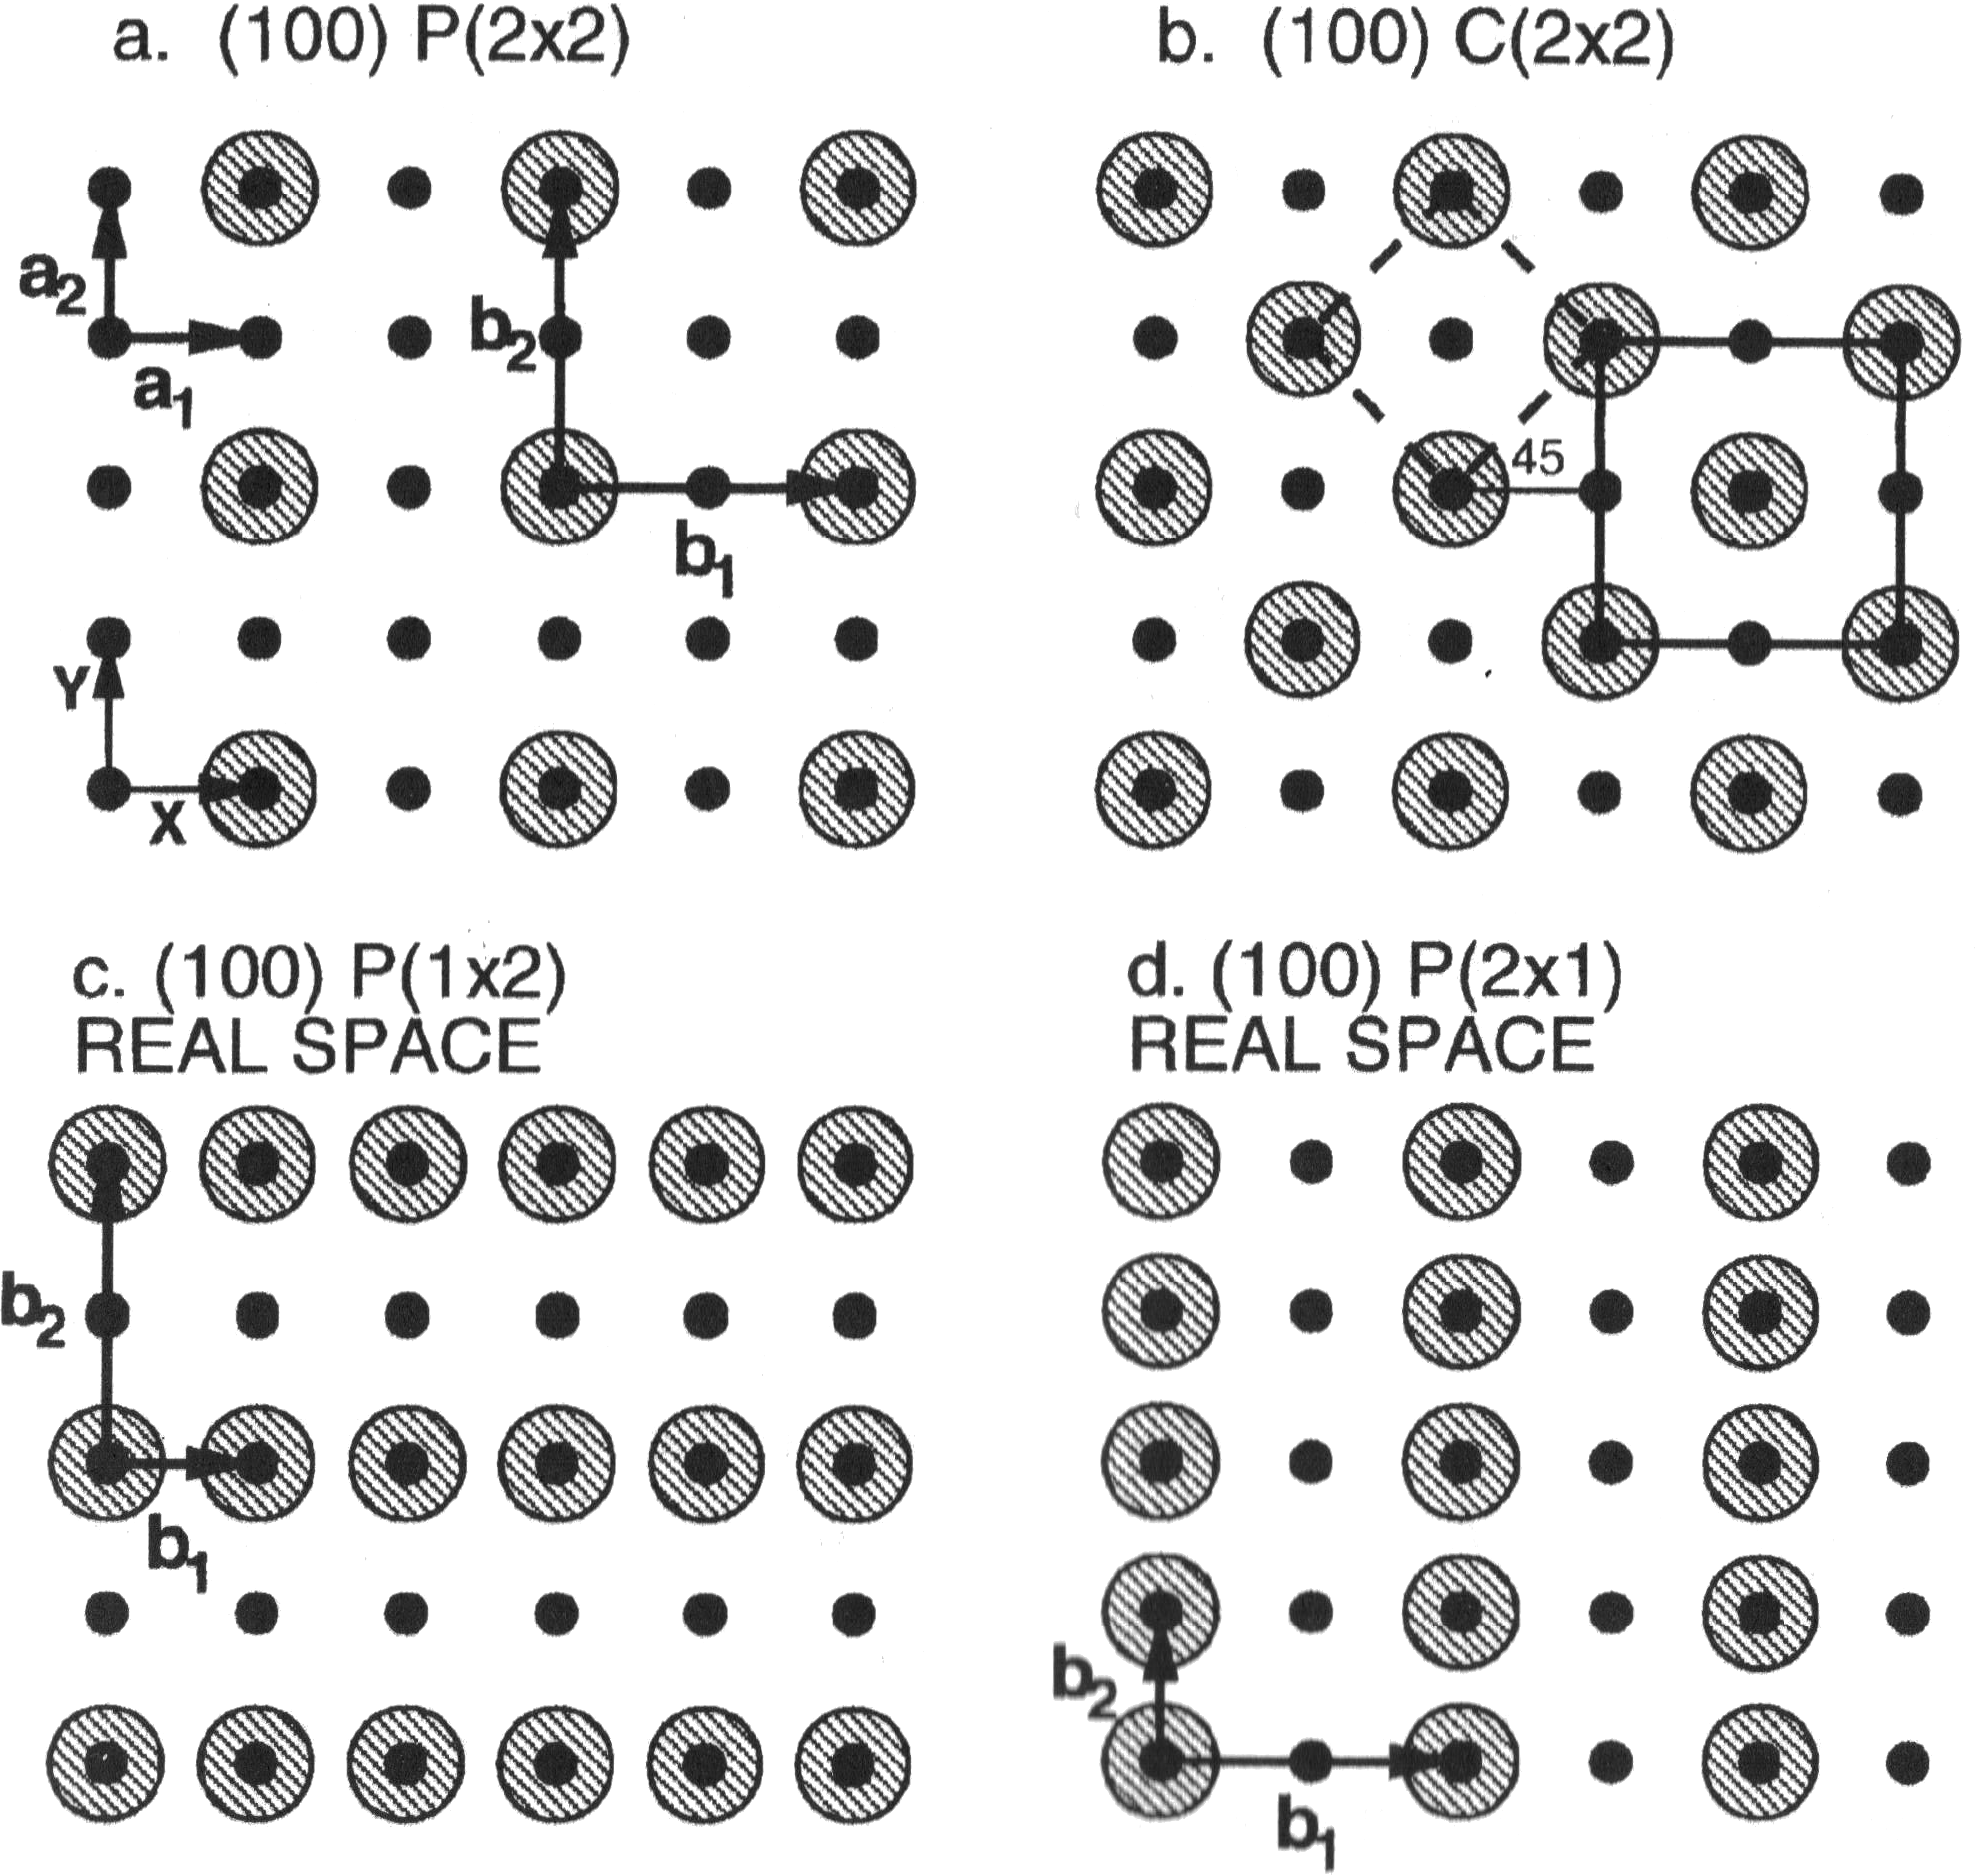
\includegraphics[width=0.9\textwidth]{back_recon_name_examples}
    \caption{\label{fig:back_recon_name_examples} Atomic positions of adatoms (shaded) relative to atoms (dots) arrayed on a (100) simple cubic substrate. a) P($2 \times 2$) b) C($2 \times 2$) or ($\sqrt{2}\times\sqrt{2}$)R45\degree c) P($1 \times 2$) d) P($2 \times 1$)}
\end{figure}

\section{Atomic Bonding}
\begin{figure}
    \centering
    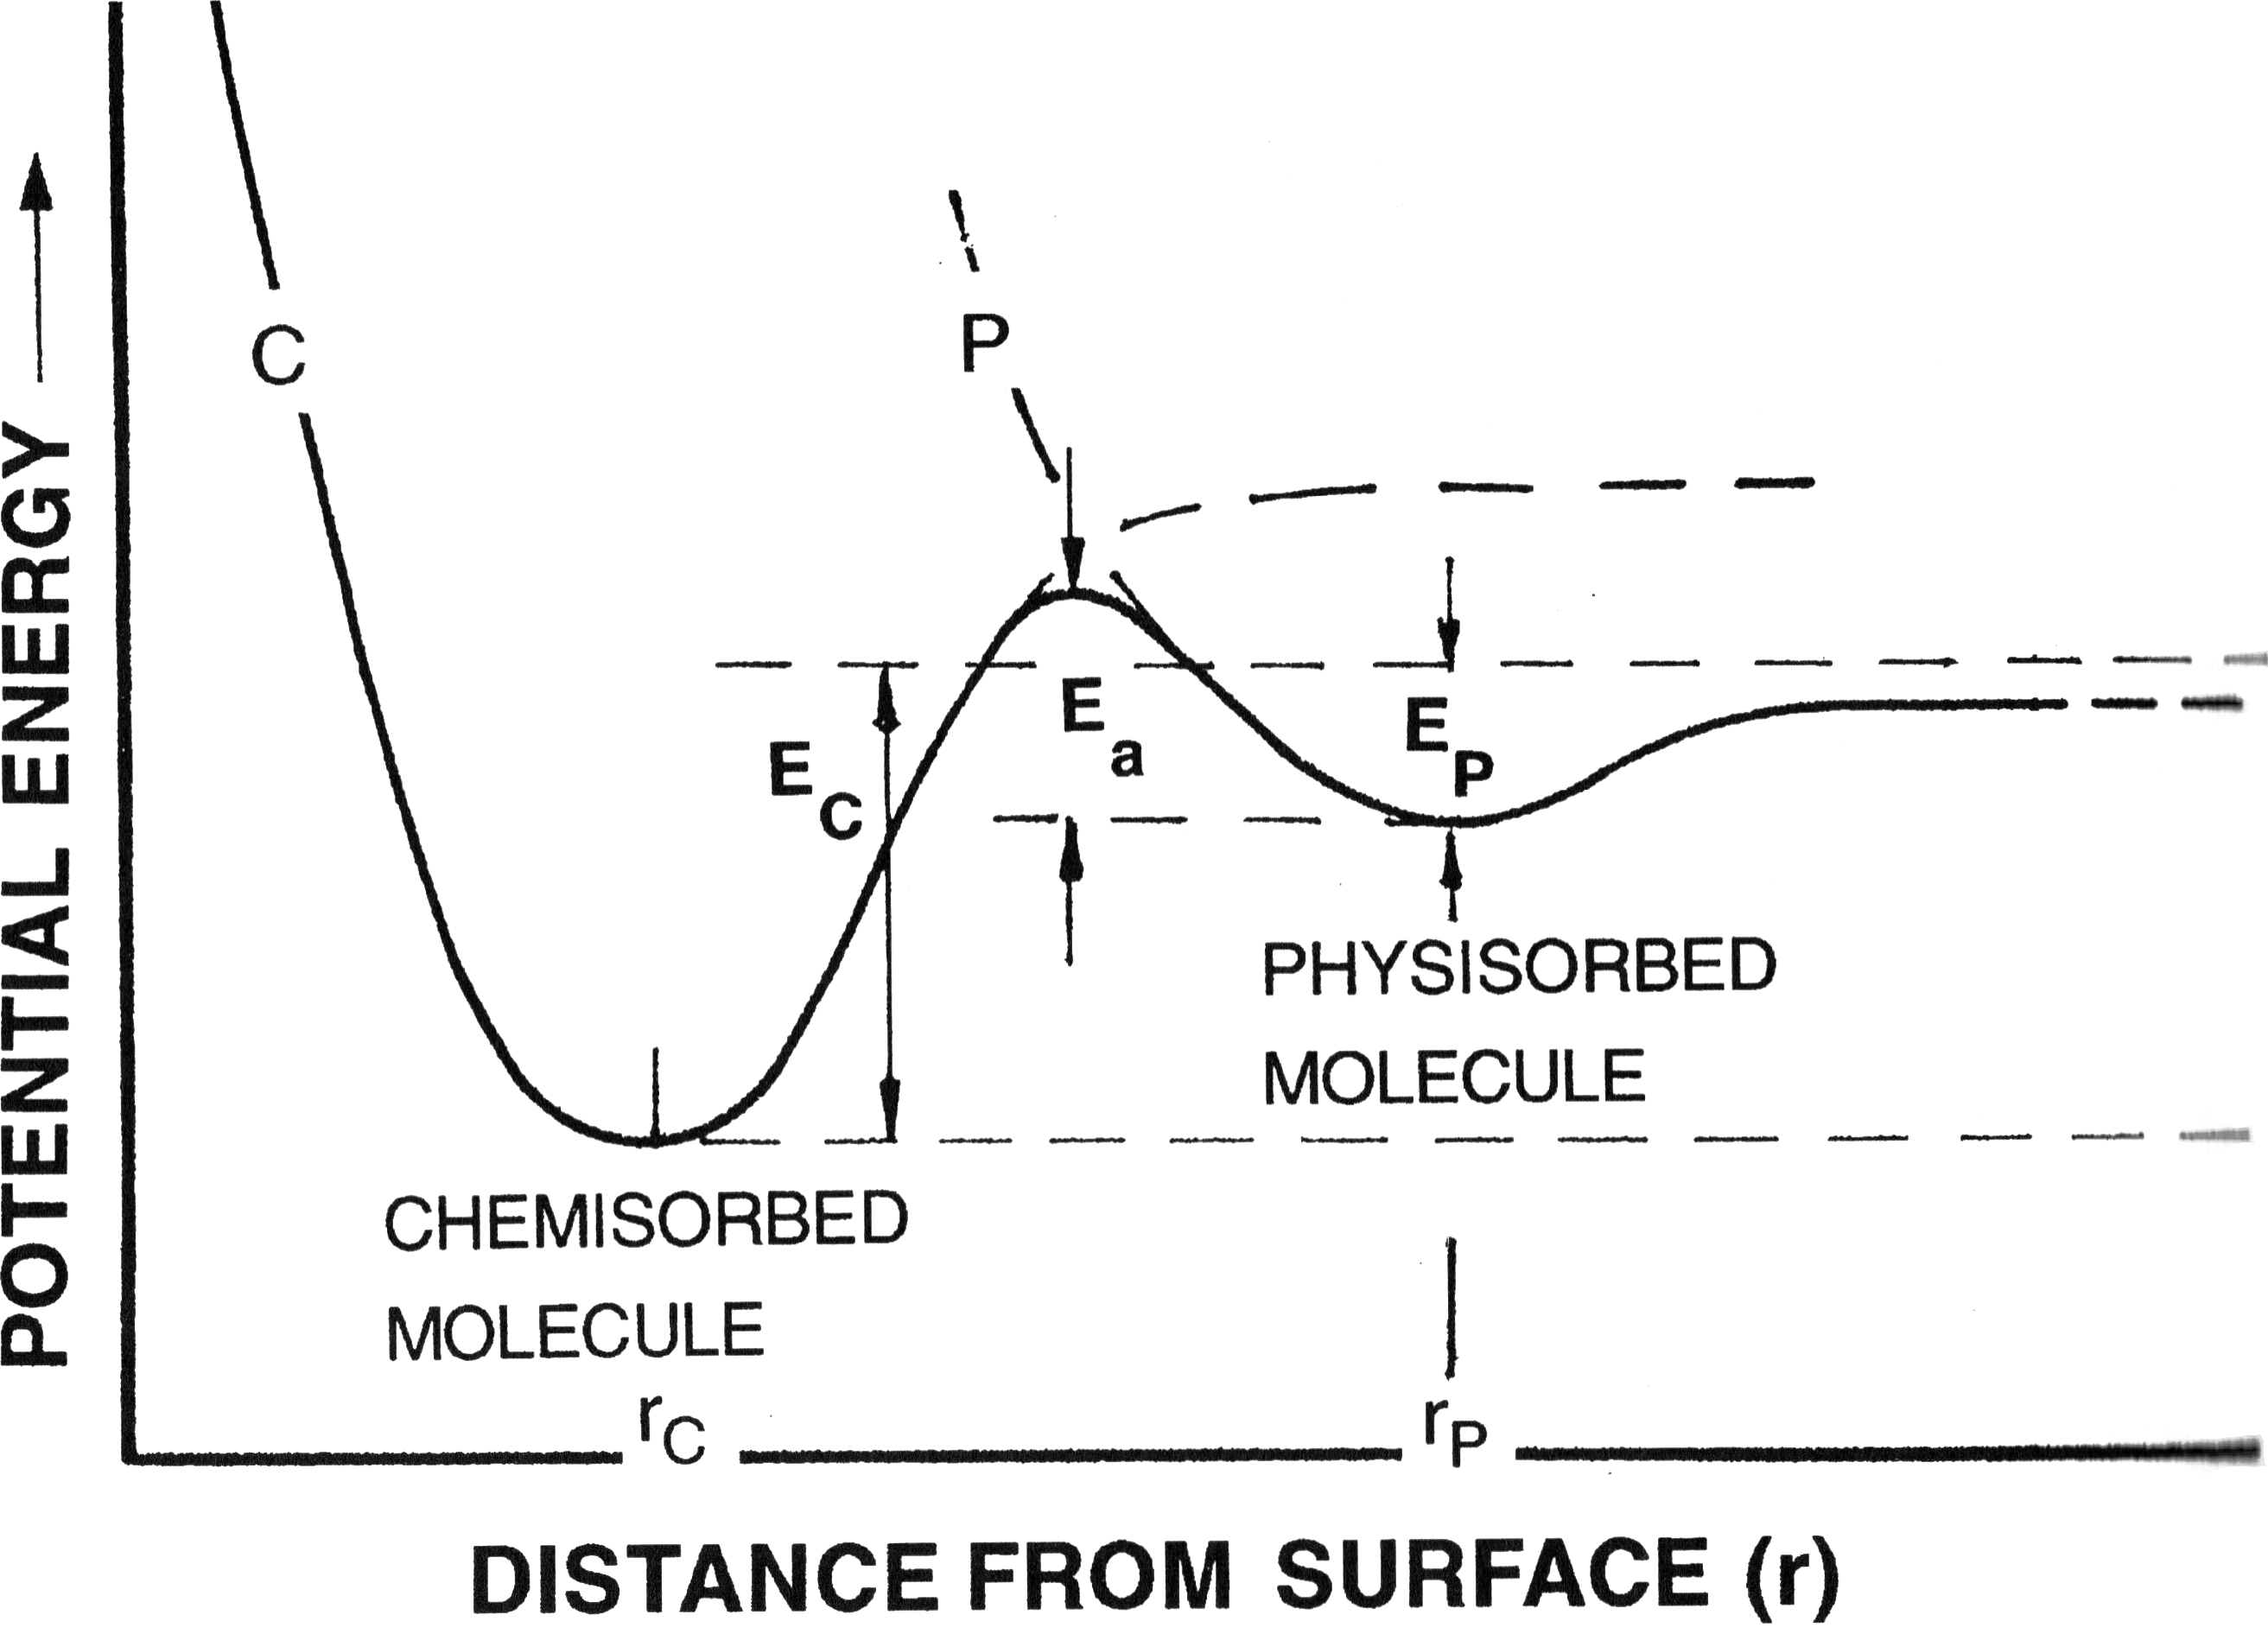
\includegraphics[width=0.9\textwidth]{back_bond_potential}
    \caption{\label{fig:back_bond_potential}Potential energy versus distance for atom respect to surface}
\end{figure}

